%
% chapter.tex -- Holomorphe Funktionen
%
% (c) 2025 Prof Dr Andreas Müller
%
% !TeX spellcheck = de_CH
\chapter{Holomorphe Funktionen
\label{chapter:holomorph}}
\kopflinks{Holomorphe Funktionen}

Komplexe Funktionen, wie sie im Kapitel~\ref{chapter:komplex} beschrieben
worden sind, scheinen soweit noch keine aussergewöhnlichen Eigenschaften
zu haben.
Einzig die Eigenschaft, dass der Fundamentalsatz zu jedem
beliebigen Polynom $K[x]$ die Existenz einer algebraischen Funktion
über $K\subset\mathbb{C}$ garantiert, kann als neue Eigenschaft im 
Komplexen angesehen werden.
Sie verwendet ausschliesslich, dass $\mathbb{C}$ algebraisch
abgeschlossen ist, es handelt sich also um eine rein algebraische
Eigenschaft.
Der Körper der komplexen Zahlen ist aber auch ein zweidimensionaler
Vektorraum $\mathbb{R}^2$, in dem die Ableitung definiert ist.
In diesem Kapitel soll die komplexe Ableitung definiert werden und
gezeigt werden, dass die Existenz der komplexen Ableitung einer 
Funktion sehr strenge zusätzliche Einschränkung auferlegt.

\def\Jf{J\!f}

%
% 1-holomorph.tex
%
% (c) 2025 Prof Dr Andreas Müller
%
\section{Holomorphe Funktionen
\label{buch:holomorph:section:holomorph}}
\kopfrechts{Holomorphe Funktionen}
In diesem Abschnitt betrachten wir eine komplexe Funktion $f$, die auf
einem Gebiet $U\subset\mathbb{C}$ definiert ist.
Wir verwenden, sofern nichts anderes vermerkt ist, die Notation
\[
f(z) = f(x+iy) = u(x,y) + iv(x,y)
\qquad
\text{mit $z=x+iy\in U$.}
\]
Die Funktionen $u$ und $v$ sind also Funktionen von zwei reellen Variablen.
Wir nehmen ausserdem an, dass $f$ und damit auch die Funktionen $u$ und $v$
stetig sind.

%
% Komplexe Differenzierbarkeit
%
\subsection{Komplexe Differenzierbarkeit
\label{buch:holomoprh:holomorph:subsection:komplexedifferenzierbarkeit}}
Im Anfängerunterricht der Analysis wird meistens der Begriff der Steigung
einer Tangente an den Graphen einer Funktion als Motivation für die Definition
der Ableitung der Funktion verwendet.
Diese geometrische Intuition funktioniert für komplexe Funktionen
nicht mehr, da der Graph einer komplexen Funktion eine Fläche in einem
vierdimensionalen reellen Vektorraum ist, der unserer Anschauung unzugänglich
ist.
Es muss daher eine rein analytische Definition gefunden werden.

%
% Ableitungen als Differenzenquotienten
%
\subsubsection{Ableitungen als Differenzenquotienten}
Die Ableitung einer reellen Funktion $f\colon I \to\mathbb{R}$ wird oft
als der Grenzwert 
\[
f'(x) = \lim_{h\to 0} \frac{f(x+h) - f(x)}{h}
\]
eingeführt.
Eine komplexe Funktion können wir als zwei reellwerte Funktionen
von \emph{zwei} reellen Variablen $x$ und $y$ betrachten, es gibt
daher die vier verschiedene reelle Ableitungen
\begin{align*}
\frac{\partial u}{\partial x}(x,y)
&=
\lim_{h\to0} \frac{u(x+h,y)-u(x,y)}{h},
&
\frac{\partial v}{\partial x}(x,y)
&=
\lim_{h\to0} \frac{v(x+h,y)-v(x,y)}{h},
\\
\frac{\partial u}{\partial y}(x,y)
&=
\lim_{h\to0} \frac{u(x,y+h)-u(x,y)}{h},
&
\frac{\partial v}{\partial y}(x,y)
&=
\lim_{h\to0} \frac{v(x,y+h)-v(x,y)}{h}.
\end{align*}
Zusammen bilden diese Ableitungen die Jacobi-Matrix
\index{Jacobi-Matrix}%
\[
\Jf(x,y)
=
\frac{\partial (u,v)}{\partial(x,y)}
=
\renewcommand{\arraystretch}{1.8}
\begin{pmatrix}
\displaystyle \frac{\partial u}{\partial x}(x,y)
&
\displaystyle \frac{\partial u}{\partial y}(x,y)
\\
\displaystyle \frac{\partial v}{\partial x}(x,y)
&
\displaystyle \frac{\partial v}{\partial y}(x,y)
\end{pmatrix}.
\]
Welche dieser partiellen Ableitungen kann die Rolle einer komplexen
Ableitung übernehmen?
Offenbar reicht die Idee des Differenzenquotienten allein nicht aus,
um eine komplexe Ableitung zu definieren.

%
% Die lineare Ersatzfunktion
%
\subsubsection{Die lineare Ersatzfunktion}
Die Ableitung kann aber auch als eine lineare Approximation
der Funktion betrachtet werden.
Für eine Funktion einer Variablen ist die Taylor-Reihe
\index{Taylor-Reihe}%
\[
f(x+h)
=
f(x)
+
f'(x) h
+
\frac{f''(x)}{2!}h^2
+
\dots
.
\]
Die Terme mindestens quadratischer Ordnung in $h$ können zusammengefasst
werden in einen Ausdruck $o(h)$ mit der Eigenschaft, dass
\[
\lim_{h\to 0}
\frac{o(h)}{h}
\]
ist.
Damit lässt sich die Taylor-Reihe schreiben als
\[
f(x+h)
=
f(x) + f'(x) h + o(h).
\]
Die ersten zwei Terme bilden eine lineare Funktion, die bis auf
die Korrektur $o(h)$ kleinerer Ordnung die Funktion $f(x+h)$
korrekt wiedergibt.
Solange man also nur eine lineare Approximation benötigt, ist
\begin{equation}
f(x+h)
\approx
f(x) + f'(x) \cdot h
\label{buch:holomorph:holomorph:1dersatz}
\end{equation}
die geeignete \emph{lineare Ersatzfunktion}.
\index{lineare Ersatzfunktion}%

Die Taylor-Reihe der als Abbildung $\mathbb{R}^2\to\mathbb{R}^2$
betrachteten komplexen Funktion $f$ ist bis zu Termen erster Ordnung
\[
f(x+\Delta x,y + \Delta y)
=
f(x,y)
+
\Jf(x,y)\begin{pmatrix}
\Delta x\\
\Delta y
\end{pmatrix}
+
o(\Delta x,\Delta y).
\]
Die lineare Ersatzfunktion
\begin{equation}
f(z+\Delta z)
\approx
f(z)
+
\Jf
\begin{pmatrix}
\Delta x \\
\Delta y
\end{pmatrix}
\label{buch:holomorph:holomorph:2dersatz}
\end{equation}
ist jetzt also durch die Jacobi-Matrix gegeben, wobei
$\Delta z = \Delta x + i \Delta y$.
Die Jacobi-Matrix muss verwendet werden, weil hier $\Delta z$ als
zweidimensionaler reeller Vektor betrachtet wird.

Für eine komplexe Funktion möchte man $\Delta z$ als einen eindimensionalen
komplexen Vektor betrachten.
Statt der Darstellung  \eqref{buch:holomorph:holomorph:2dersatz} der
linearen Ersatzfunktion möchte man eine Formel haben, welche wie
\eqref{buch:holomorph:holomorph:1dersatz} aussieht.
Wir erwarten also, dass es eine lineare Ersatzfunktion der Form
\[
f(z+\Delta z)
=
f(z) + f'(z)\Delta z
+
o(\Delta z)
\]
mit einer komplexen Zahl $f'(z)\in\mathbb{C}$ gibt.
Falls dies möglich ist, betrachten wir $f'(z)$ als die
komplexe Ableitung von $f'(z)$.

\begin{definition}[komplexe Ableitung]
\label{buch:holomorph:diffbar:def:komplexeableitung}
Sei $f(z)$ eine komplexe Funktion.
Die \emph{komplexe Ableitung} $f'(z)$ von $f$ im Punkt
\index{komplexe Ableitung}%
$z\in\mathbb{C}$ ist die komplexe Zahl, für die $f(z) + f'(z) \Delta z$
die lineare Ersatzfunktion von $f(z+\Delta z)$ ist.
\end{definition}

\begin{definition}[holomorphe Funktion]
\index{holomorph}%
Eine komplexe Funktion $f\colon U\to\mathbb{C}$ heisst \emph{holomorph},
wenn sie in $U$ eine komplexe Ableitung besitzt.
\end{definition}

Die lineare Funktion $f(z) = az+b$ ist ihre eigene lineare Ersatzfunktion,
es gibt also mindestens diese eine holomorphe Funktion mit der komplexen
Ableitung $f'(z)=a$.
Es ist aber nicht klar, ob Forderung nach einer linearen Ersatzfunktion
vielleicht zu streng ist und nicht viele holomorphe Funktionen übrig
bleiben.
Als nächstes müssen wir uns also mit der Frage nach der Berechnung der
komplexen Ableitung befassen.

%
% Berechnung der komplexen Ableitung
%
\subsubsection{Berechnung der komplexen Ableitung}
Da die komplexe Ableitung $f'(z)$ einer holomorphen Funktion im Punkt $z$
die komplexe lineare Ersatzfunktion 
\[
f(z+h) = f(x) + f'(z)\cdot h + o(h)
\]
definiert, wobei $h\in\mathbb{C}$ beliebig ist, kann man sie auch als
Grenzwert
\[
\lim_{h\to 0}
\frac{f(z+h)-f(z)}{h}
=
f'(z)
\]
berechnen.
Im Grenzübergang dürfen auch spezielle Werte für $h$ verwendet werden,
zum Beispiel könnte die Ableitung mit
\begin{align}
f'(z)
&=
\lim_{x\to 0}
\frac{f(z+x)-f(z)}{x}
&&\text{oder}&
f'(z)
&=
\lim_{y\to 0}
\frac{f(z+iy)-f(z)}{iy}
\label{buch:holomorph:holomorph:eqn:ablxy}
\end{align}
gefunden werden, wobei der Grenzübergang für $x$ oder $y$ in $\mathbb{R}$
erfolgt.

\begin{lemma}
\label{buch:holomorph:holomorph:lemma:reellnichtholomorph}
Ist $f(z)$ eine komplexe Funktion mit ausschliesslich reellen Werten,
dann ist sie nicht holomorph.
Eine komplexe Funktion mit ausschliesslich imaginären Werten ist
nicht holomorph.
\end{lemma}

\begin{proof}
Wenn $f(z)$ nur reelle Werte hat, dann ist der linke Grenzwert in
\eqref{buch:holomorph:holomorph:eqn:ablxy} 
ein Grenzwert in $\mathbb{R}$.
Der rechte Grenzwert in
\eqref{buch:holomorph:holomorph:eqn:ablxy} 
dagegen ist wegen $1/i=-i$ ein Grenzwert in
den imaginären Zahlen $i\mathbb{R}\subset\mathbb{C}$.
Somit muss 
\[
f'(z) \in \mathbb{R} \cap i\mathbb{R} = \{0\}
\qquad\Rightarrow\qquad
f'(z) = 0
\]
gelten.
\end{proof}

Die Differenzenquotienten in \eqref{buch:holomorph:holomorph:eqn:ablxy}
können auch als partielle Ableitungen nach $x$ bzw.~$y$ betrachtet werden,
es folgt daher auch
\begin{equation}
\begin{aligned}
f'(z)
&=
\frac{\partial u}{\partial x}(x,y)
+
i\frac{\partial v}{\partial x}(x,y)
\quad\text{und}
\\
f'(z)
&=
\frac{1}{i}
\biggl(
\frac{\partial u}{\partial y}(x,y)
+
i
\frac{\partial v}{\partial y}(x,y)
\biggr)
=
\frac{\partial v}{\partial y}(x,y)
-
i\frac{\partial u}{\partial y}(x,y).
\end{aligned}
\label{buch:holomorph:holomorph:eqn:kablpart}
\end{equation}
Dies deutet bereits an, dass die komplexe Ableitung mit nur einem
Paar von reellen Ableitungen berechnet werden kann.
Es muss also einen Zusammenhang zwischen den vier partiellen
Ableitungen der beiden Funktionen $u$ und $v$ geben, der weiter
unten im Satz~\ref{buch:holomorph:holomorph:satz:cr} formalisiert
wird.

Der Real- und Imaginärteil der Ableitung lässt sich allein aus dem
Real- und Imaginärteil der Funktion bestimmen.
Es ist nämlich
\begin{align*}
f'(z)
&=
\frac{\partial u}{\partial x}(x,y) + i\frac{\partial v}{\partial x}(x,y).
\intertext{Also folgt}
\operatorname{Re}f'(z)
&=
\frac{\partial u}{\partial x}(x,y)
=
\frac{\partial}{\partial x} \operatorname{Re} f(z)
&&\text{und}&
\operatorname{Im}f'(z)
&=
\frac{\partial v}{\partial x}(x,y)
=
\frac{\partial}{\partial y} \operatorname{Im} f(z).
\end{align*}
Man beachte aber, dass die reellwertigen Funktionen $\operatorname{Re}f(z)$
und $\operatorname{Im}f(z)$ nach
Lemma~\ref{buch:holomorph:holomorph:lemma:reellnichtholomorph}
keine komplexe Ableitung haben, es ist also
nicht zulässig, $\operatorname{Re} f(z) = \frac{d}{dz}\operatorname{Re}f(z)$
zu schreiben, da die Schreibweise $\operatorname{Re}f(z)$ den Realteil
als eine komplexe Funktion ausweist.

%
% Ableitungsregeln
%
\subsubsection{Ableitungsregeln}
In der Praxis berechnet man die Ableitung einer Funktion mestens nicht
mit einem Grenzübergang sondern viel erfolgreicher und vor allem schneller
durch Anwendung algebraischer Regeln.
Diese Regeln bleiben auch für holomorphe Funktionen gültig.
\index{Ableitungsregeln}%

\begin{satz}[Rechenregeln]
\label{buch:holomorph:holomorph:satz:rechenregeln}
Seien $f(z)$ und $g(z)$ holomorphe Funktionen.
\begin{enumerate}
\item Die komplexe Ableitung ist ein linearer Operator
\[
\frac{d}{dz} \bigl(\lambda f(z) + \mu g(z)\bigr)
=
\lambda \frac{df}{dz}(z) + \mu\frac{dg}{dz}(z)
=
\lambda f'(z) + \mu g'(z).
\]
\index{linear}%
\item Es gilt die Produktregel
\[
\frac{d}{dz}\bigl(f(z)g(z))
=
f'(z)g(z) + f(z)g'(z).
\]
\index{Produktregel}%
\item
Falls $g(z)\ne 0$ gilt die Quotientenregel
\[
\frac{d}{dz}\biggl(\frac{f(z)}{g(z)}\biggr)
=
\frac{f'(z)g(z)-f(z)g'(z)}{g(z)^2}.
\]
\item Es gilt die Kettenregel
\[
\frac{d}{dz}
(f\circ g)(z)
=
\frac{d}{dz}
f(g(z))
=
f'(g(z)) g'(z)
\]
\index{Quotientenregel}%
\item Die Ableitung der zu $f$ inversen Funktion $f^{-1}(z)$ ist
\begin{equation}
\frac{d}{dz} f^{-1}(z)
=
\frac{1}{f'(f^{-1}(z))}.
\label{buch:holomoroph:holomorph:eqn:inverseholomorph}
\end{equation}
\index{Ableitung der inversen Funktion}%
\index{inverse Funktion, Ableitung}%
\end{enumerate}
\end{satz}

\begin{proof}
\begin{enumerate}
\item
Die Linearität folgt sofort aus
\eqref{buch:holomorph:holomorph:eqn:kablpart}
der Linearität der partiellen Ableitungen.
\index{Linearität}%
\item
Es genügt die Ableitung nach $x$ zu betrachten, also
\begin{align*}
\frac{d}{dz}(f(z)g(z))
&=
\frac{\partial}{\partial x}(u_fu_g - v_fv_g)
+
i
\frac{\partial}{\partial x}(u_fv_g + v_fu_g,
\intertext{wobei $f(z) = u_f + iv_f$ und $g(z) = u_g+iv_g$.
Für jedes Produkt reeller Funktionen gilt die Produktregel, wir erhalten}
&=
\frac{\partial u_f}{\partial x}
u_g
+
u_f
\frac{\partial u_g}{\partial x}
-
\frac{\partial v_f}{\partial x}
v_g
-
v_f
\frac{\partial v_g}{\partial x}
\\
&\qquad
+i
\biggl(
\frac{\partial u_f}{\partial x}
v_g
+
u_f
\frac{\partial v_g}{\partial x}
+
\frac{\partial v_f}{\partial x}
u_g
+
v_f
\frac{\partial u_g}{\partial x}
\biggr)
\\
&=
\frac{\partial u_f}{\partial x}
u_g
-
\frac{\partial v_f}{\partial x}
v_g
+i
\biggl(
\frac{\partial u_f}{\partial x}
v_g
+
\frac{\partial v_f}{\partial x}
u_g
\biggr)
\\
&\qquad
+
u_f
\frac{\partial u_g}{\partial x}
-
v_f
\frac{\partial v_g}{\partial x}
+
i
\biggl(
u_f
\frac{\partial v_g}{\partial x}
+
v_f
\frac{\partial u_g}{\partial x}
\biggr)
\\
&=
\biggl(
\frac{\partial u_f}{\partial x}
+i
\frac{\partial v_f}{\partial x}
\biggr)
(u_g+iv_g)
+
(u_f+iv_f)
\biggl(
\frac{\partial u_g}{\partial x}
+i
\frac{\partial v_g}{\partial x}
\biggr)
\\
&=
f'(z)g(z) + f(z)g'(z).
\end{align*}
\index{Produktregel}%
\item
Wir schreiben $h(z) = f(z)/g(z)$.
Wir müssen also $h'(z)$ berechnen.
Dazu leiten wir die Identität $f(z) = h(z) g(z)$ nach $z$ ab und
erhalten nach der Produktregel
\begin{align*}
f'(z) &= h'(z) g(z) + h(z) g'(z) = h'(z) g(z) + \frac{f(z)}{g(z)}g'(z).
\intertext{Auflösen nach $h'(z)$ ergibt}
h'(z)g(z)
&=
f'(z)-\frac{f(z)g'(z)}{g(z)}
\\
h'(z)
&=
\frac{f'(z)}{g(z)}-\frac{f(z)g'(z)}{g(z)^2}
\intertext{oder durch gleichnamig Machen}
h'(z)
&=
\frac{f'(z)g(z) - f(z)g'(z)}{g(z)^2},
\end{align*}
die Quotientenregel.
\index{Quotientenregel}%
\item
Die Zusammensetzung $f^{-1}\circ f$ ist die Identität
\(
z = f^{-1}(f(z))
\)
und hat wegen der Kettenregel die Ableitung
\[
1
=
\frac{d}{dz}
f^{-1}(f(z))
=
f^{-1\prime}(f(z)) f'(z).
\]
Aufgelöst nach der Ableitung von $f^{-1}$ folgt
\[
f^{-1\prime}(f(z))
=
\frac{1}{f'(z))}.
\]
Um die Ableitung an der Stelle $z$ statt $f(z)$ zu bekommen, muss man 
$z$ durch $f^{-1}(z)$ ersetzen, was
\[
f^{-1\prime}(z)
=
f^{-1\prime}(f(f^{-1}(z)))
=
\frac{1}{f'(f^{-1}(z))}
\]
und damit die Behauptung ergibt.
\qedhere
\end{enumerate}
\end{proof}

Der Satz zeigt, dass all die bekannten Ableitungsregeln aus der
reellen Analysis weiterhin gelten, wenn man sie als komplexe
Ableitungen interpretiert.
Mit den Ableitungsregeln lassen sich jetzt weitere bekannten Ableitungsformeln
für komplexe Ableitungen reproduzieren.
Der Beweis zeigt auch, dass vor allem Linearität und die Produktregel
ausschlaggebend sind, wie weiteren Regeln folgen daraus automatisch.
Wir werden auf diese zentrale Bedeutung der Produktregel in
Abschnitt~\ref{buch:intalg:section:elementar} zurückkommen.

\begin{beispiel}
Sie $f(z)=z^n$, dann ist
\begin{equation}
f'(z) = nz^{n-1}.
\label{buch:holomorph:holomorph:bsp:eqn:zn}
\end{equation}
Der Fall $n=1$ ist der bereits bekannte lineare Fall, in diesem Fall
stimmt die Formel.
Wir verwenden daher vollständige Induktion und nehmen an, das die Formel
\eqref{buch:holomorph:holomorph:bsp:eqn:zn}
für $n-1$ bereits bewiesen ist.
Nach der Produktregel ist
\begin{align*}
\frac{d}{dz}
z^n
&=
\frac{d}{dz}\bigl(z\cdot z^{n-1}\bigr)
=
\biggl(\frac{d}{dz} z\biggr)\cdot z^{n-1}
+
z\cdot\biggl( \frac{d}{dz} z^{n-1}\biggr)
\intertext{Die Ableitungen können mit der Induktionsannahme berechnet 
werden und es ergibt sich}
&=
1\cdot z^{n-1}
+
z\cdot(n-1)z^{n-2}
\\
&=
z^{n-1} + (n-1)z^{n-1}
=
nz^{n-1}.
\end{align*}
Damit ist die Ableitungsformel bewiesen.
\end{beispiel}

%
% Die Stammfunktion
%
\subsubsection{Die Stammfunktion}
Der Hauptsatz der Infinitesimalrechnung besagt, dass Differenzieren und
Integrieren zueinander inverse Operationen sind.
Dies ermöglicht, Integrale mithilfe einer Stammfunktion zu berechnen.
Für komplexe Funktionen steht uns vorerst noch kein Integralbegriff
zur Verfügung, aber die Idee der Stammfunktion lässt sich leicht auf
komplexe Funktionen übertragen.

\begin{definition}[Stammfunktion]
\index{Stammfunktion}%
Eine \emph{Stammfunktion} einer stetigen komplexen Funktion $f(z)$
ist eine holomorphe Funktion $F(z)$ derart, dass $F'(z) = f(z)$.
\end{definition}

Man beachte, dass die Stammfunktion ganz ohne Bezug auf das
Integral definiert wurde.
Nichtsdestotrotz wird eine Stammfunktion manchmal auch $\int f$
geschrieben.
Diese algebraische Betrachtungsweise ist insbesondere unabhängig
von den analytischen Eigenschaften der komplexen Zahlen.

\begin{definition}[Stammfunktion, algebraische Definition]
Sei $K$ ein Körper von Funktionen der unabhängigen Variable $z$ und
$f\in K$.
Dann heisst $F\in K$ eine Stammfunktion von $f$, wenn $F'=f$ gilt.
\end{definition}

Aus den Ableitungsregeln für holomorphe Funktionen folgen unmittelbar
die folgenden Rechenregeln für Stammfunktionen:
\begin{enumerate}
\item
\(\displaystyle
\int z^n = \frac{1}{n+1} z^{n+1}
\)
für $n\in\mathbb{Z}, n\ne -1$.
\item Partielle Integration:
\(\displaystyle
\int f'g
=
fg
-
\int fg'.
\)
\end{enumerate}

Die Stammfunktion ist im Allgemeinen nur bis auf eine Konstante
definiert.
Dabei stellen wir uns eine Konstante typischerweise als etwas
vor, was nicht von der unabhängigen Variable abhängt.
Der Ausdruck $f(z)=(1+z)^2-z^2-2z$ scheint von $z$ abzuhängen,
doch wenn man die Klammer ausmultipliziert bleibt $f(z)=1$ übrig.
In diesem speziellen Fall war es einfach zu erkennen, dass die Abhängigkeit
von $z$ nur scheinbar ist.
Im Allgemeinen ist es ein nicht entscheidbares Problem, herauszufinden,
ob ein Ausdruck verschwindet.
Wir benötigen daher eine Definition für Konstanten, die sich nicht
auf die syntaktische Form eines Ausdrucks bezieht, sondern nur 
algebraische Eigenschaften verwendet.
Dies führt auf die folgende, leicht zirkuläre Definition.

\begin{definition}[Konstante]
Eine \emph{Konstante} in einem Funktionenkörper ist ein Element $c\in K$
\index{Konstante}%
mit der Eigenschaft $c'=0$.
\end{definition}

Übrigens lässt sich auch die unabhängige Variable $z$ rein aus
algebraischen Eigenschaften des Ableitunsgoperators rekonstruieren.
Die unabhängige Variable $z$ ist eine Stammfunktion der Funktion $1$.
In diesem Lichte ist die unabhängige Variable $z$ nur bis auf eine
Konstante bestimmt.
Funktionen sind damit nur bis auf eine ``Verschiebung'' festgelegt.


%
% Der Mittelwertsatz
%
\subsubsection{Der Mittelwertsatz}
In der reellen Analysis gilt der folgende, aus der Anschauung von
Abbildung~\ref{buch:holomorph:fig:mittelwert} plausible Mittelwertsatz.
%
% fig-mittelwert.tex -- Abbildung zum Mittelwertsatz
%
% (c) 2026 Prof Dr Andreas Müller
%
\begin{figure}
\centering
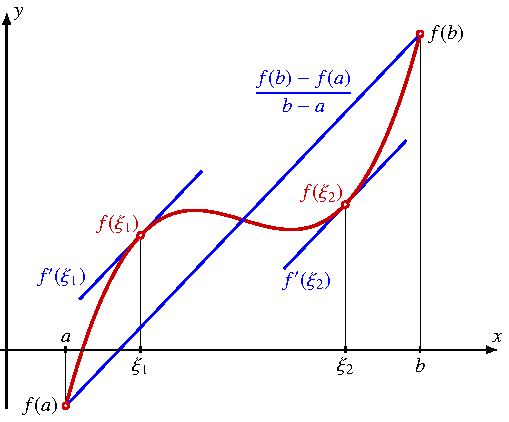
\includegraphics{chapters/020-holomorph/images/mittelwert.pdf}
\caption{Der Mittelwertsatz für eine reelle, differenzierbare Funktion
besagt, dass es zu zwei Werten $a$ und $b$ immer mindestens einen
Zwischenwert $\xi$ gibt, in dem die Steigung von $f(x)$ mit dem
der Sekantensteigung zwischen den Punkten $(a,f(a))$ und $(b,f(b))$
übereinstimmt.
\label{buch:holomorph:fig:mittelwert}}
\end{figure}
%

\begin{satz}[Mittelwertsatz]
\index{Mittelwertsatz}%
Ist $f\colon I \to \mathbb{R}$ eine stetig differenzierbare Funktion auf
dem Intervall $I=[a,b]$, dann gibt es ein $\xi \in I$ derart, dass
\[
f'(\xi)
=
\frac{f(b)-f(a)}{b-a}.
\]
\end{satz}

In dieser Form hängt er mit dem Zwischenwertsatz zusammen, der
Aussage, dass es für eine stetige Funktion $f$ für ein $\eta\in [f(a),f(b)]$
eine Stelle $\xi\in[a,b]$ geben muss, für die $f(\xi)=\eta$ ist.
So eine Aussage kann für komplexe Funktionen nur schon deshalb nicht
gelten, weil es im Komplexen keine Ordnungsrelation gibt.

Man kann den Mittelwertsatz aber auch als die Aussage sehen, dass 
die Funktionswerte an den Endpunkten des Intervalls nicht zu weit
auseinander liegen können, wenn die Ableitung klein ist.
In dieser Form gilt der Mittelwertsatz auch für Funktionen
mehrerer Variablen, braucht dazu aber das Konzept der Norm einer
linearen Abbildung.

\begin{definition}[Norm]
\index{Norm}%
Sei $A\colon \mathbb{R}^n\to\mathbb{R}^m$ eine lineare Abbildung.
Die \emph{Norm} von $A$ ist
\[
\| A\|
=
\sup_{x\in\mathbb{R}^n\setminus\{0\}} \frac{|Ax|}{|x|}.
\]
\end{definition}

Die Norm von $\|A\|$ ist auch der maximale Wert, den $|A|$ für 
Vektoren $x$ auf der Einheitskugel in $\mathbb{R}^n$ annimmt.
Der Mittelwertsatz lautet damit jetzt wie folgt.

\begin{satz}[Mittelwertsatz]
\index{Mittelwertsatz}%
Sei $U\subset \mathbb{R}^n$ ein Gebiet in $\mathbb{R}^n$ und seien
$x_0\in U$ und $x_0+t\in U$ zwei Punkte in $U$ derart, dass auch
die Verbindungsstrecke in $U$ enthalten ist.
Dann gilt
\[
|f(x_0+t) - f(x_0)|
\le
|t|\cdot \sup_{0\le \xi \le 1} \| \Jf(x_0+\xi t) \|,
\]
wobei $\Jf$ die $m\times n$-Jacobi-Matrix
\[
\Jf(x) = \frac{\partial (f_1,\dots,f_m)}{\partial(x_1,\dots,x_n)}
\]
ist.
\end{satz}

Für eine komplexe Funktion nimmt dieser Satz eine besonders einfach
Form an, weil die Ableitung von $f$ durch eine einzige komplexe
Zahl beschrieben wird.
Die Norm der Ableitung ist
\[
\| \Jf(z) \|
=
\sup_{|w|=1} | f'(z)\cdot w |
=
\sup_{|w|=1} |f'(z)| \cdot |w|
=
|f'(z)|.
\]
Die Norm ist also nichts anderes als der Betrag der komplexen 
Ableitung.
Der Mittelwertsatz für komplexe Funktionen lautet daher wie folgt.

\begin{satz}[Mittelwertsatz für holomorphe Funktionen]
\index{Mittelwertsatz}%
Sei $f$ eine in $U$ holomorphe Funktion und $z_0$ und $z_0+t$ Punkte
in $U$ derart, dass auch ihre Verbindungsstrecke in $U$ enthalten ist.
Dann gilt
\[
|f(z_0+t) - f(x_0)|
\le 
|t| \sup_{0\le \xi \le1}  |f'(z_0+\xi t)|.
\]
\end{satz}

Der Satz besagt also, dass der Abstand des Funktionswert $f(z_0+t)$
von $f(z_0)$ durch die Ableitung $f'(z)$ auf der Strecke zwischen
$z_0+t$ und $z_0$ und durch die Länge der Strecke beschränkt ist.
Er ist das zentrale Werkzeug um zu beweisen, dass die Ableitung einer
gleichmässig konvergierenden Funktionenreihe gliedweise gebildet
werden kann, wenn die abgeleitete Reihe konvergiert.
Dies wird im Abschnitt~\ref{buch:holomorph:holomorph:subsection:potenzreihen}
benötigt um zu zeigen, dass sich konvergente Potenzreihen gliedweise
ableiten lassen.

%
% Ableitung algebraischer Funktionen
%
\subsubsection{Ableitung algebraischer Funktionen}
Sei $f(z)$ eine über dem Funktionenkörper $K$ algebraische Funktion
\index{algebraische Funktion, Ableitung}
mit dem Minimalpolynom
\index{Minimalpolynom}%
\[
a(X)
=
a_n(z)X^n + a_{n-1}(z)X^{n-1}+\dots a_1(z)X + a_0(z).
\]
Dann gilt die Gleichung
\begin{equation}
a_n(z)f(z)^n
+
a_{n-1}(z)f(z)^{n-1}
+
\dots
+
a_1(z) f(z)
+
a_0(z).
\label{buch:holomorph:holomorph:eqn:algebraisch}
\end{equation}
Nehmen wir zusätzlich an, dass alle Funktionen in $K$ holomorph sind,
dann können wir 
\eqref{buch:holomorph:holomorph:eqn:algebraisch}
differenzieren.
Nach der Produkt- und der Kettenregel wird aus dem Term $a_k(z)f(z)^k$
\[
\frac{d}{dz}
a_k(z)f(z)^k
=
a_k'(z) f(z)^k
+
a_k(z)kf'(z)f(z)^{k-1}.
\]
Fassen wir in der Ableitung von
\eqref{buch:holomorph:holomorph:eqn:algebraisch}
die Terme mit und ohne $f'(z)$ zusammen, erhalten wir
\begin{align}
0
&=
a_n'(z)f(z)^n+\dots a_1'f(z)+a_0'(z)
+
\bigl(
a_n(z)nf(z)^{n-1}
+
\dots
+
a_1(z)
\bigr)
f'(z),
\notag
\intertext{die wir nach $f'(z)$ auflösen können:}
f'(z)
&=
\frac{
a_n'(z)f(z)^n+\dots a_1'f(z)+a_0'(z)
}{
a_n(z)nf(z)^{n-1}
+
\dots
+
a_1(z)
}.
\label{buch:holomorph:holomorph:eqn:ablalg}
\end{align}
Der Nenner auf der rechten Seite von
\eqref{buch:holomorph:holomorph:eqn:ablalg}
kann nicht identisch verschwinden, denn dann wäre der Nenner
ein Polynom kleineren Grades, welches die algebraische Funktion
$f(z)$ bereits definiert, im Widerspruch zur Annahme, dass $a(X)$
das Minimalpolynom war.

\begin{satz}[Ableitung algebraischer Funktionen]
\label{buch:holomorph:holomorph:satz:holoalg}
Ist $f(z)$ eine über einem Körper $K$ von holomorphen Funktionen
algebraische Funktion, dann ist $f(z)$ holomorph und die Ableitung ist
durch
\eqref{buch:holomorph:holomorph:eqn:ablalg}
gegeben.
\end{satz}

\begin{beispiel}
Die Kubikwurzel einer komplexen Zahl ist algebraisch mit dem Minimalpolynom
\index{Kubikwurzel}%
$a(X)=X^3-z$.
Nach dem Satz~\ref{buch:holomorph:holomorph:satz:holoalg} ist eine
Kubikwurzel holomorph und und nach der Formel
\eqref{buch:holomorph:holomorph:eqn:ablalg}
gilt
\[
\frac{d}{dz}
\!\sqrt[3]{z}
=
\frac{-1}{3(\!\sqrt[3]{z})^2},
\]
was der aus der reellen Analysis bekannten Formel $-\frac13z^{-\frac23}$ 
entspricht.
\end{beispiel}


%
% Die Cauchy-Riemann-Differentialgleichungen
%
\subsection{Cauchy-Riemann-Differentialgleichung}
Die komplexe Ableitung $f'(z)$ einer komplexen Funktion $f(z)$
nach Definition~\ref{buch:holomorph:diffbar:def:komplexeableitung}
ist eine komplexe Zahl, mit der $\Delta z$ multipliziert werden muss.
Diese Multiplikation kann als Multiplikation der Matrix
\[
\begin{pmatrix}
\operatorname{Re}f'(z)
&
-\operatorname{Im}f'(z)
\\
\operatorname{Im}f'(z)
&
\phantom{-}\operatorname{Re}f'(z)
\end{pmatrix}
\qquad\text{mit}\qquad
\begin{pmatrix}
\operatorname{Re}\Delta z\\
\operatorname{Im}\Delta z
\end{pmatrix}
\]
betrachtet werden.

Andererseits zeigt \eqref{buch:holomorph:holomorph:2dersatz},
dass diese Matrix auch mit der Jacobi-Matrix der Funktion $f$
betrachtet als einer vektorwertigen Funktion von zwei reellen Variablen
übereinstimmen muss.
Es gilt also
\[
\begin{pmatrix}
\operatorname{Re}f'(z)
&
-\operatorname{Im}f'(z)
\\
\operatorname{Im}f'(z)
&
\phantom{-}\operatorname{Re}f'(z)
\end{pmatrix}
=
\Jf
=
\renewcommand{\arraystretch}{1.8}
\begin{pmatrix}
\displaystyle \frac{\partial u}{\partial x}(x,y)
&
\displaystyle \frac{\partial u}{\partial y}(x,y)
\\
\displaystyle \frac{\partial v}{\partial x}(x,y)
&
\displaystyle \frac{\partial v}{\partial y}(x,y)
\end{pmatrix}.
\]
Insbesondere gilt
\begin{align*}
\frac{\partial u}{\partial x}(x,y)
&=
\operatorname{Re}f'(z)
=
\frac{\partial v}{\partial y}(x,y)
&&\text{und}&
-\frac{\partial u}{\partial y}(x,y)
&=
\operatorname{Im}f'(z)
=
\frac{\partial v}{\partial x}(x,y)
\end{align*}
Dies sind zwei partielle Differentialgleichungen für Real- und Imaginärteil
einer holomorphen Funktionen.

\begin{satz}[Cauchy-Riemann-Differentialgleichungen]
\label{buch:holomorph:holomorph:satz:cr}
Realteil $u(x,y)=\operatorname{Re}f(x+iy)$ und
Imaginärteil $v(x,y)=\operatorname{Im}f(x+iy)$
einer in $U\subset \mathbb{R}$ holomorphen Funktion $f(z)$ erfüllen die
partiellen Differentialgleichungen
\begin{align}
\frac{\partial u}{\partial x}
&=
\frac{\partial v}{\partial y}
&&\text{und}&
\frac{\partial u}{\partial y}
&=
-
\frac{\partial v}{\partial x}.
\label{buch:holomorph:holomorph:eqn:cr}
\end{align}
Sie heissen die \emph{Cauchy-Riemann-Differentialgleichungen}.
\index{Cauchy-Riemann-Differentialgleichungen}%
\end{satz}

%
% Harmonische Funktionen
%
\subsubsection{Harmonische Funktionen}
Der Laplace-Operator einer Funktion $u(x_1,\dots,x_n)$ von $n$
\index{Laplace-Operator}%
reellen Variablen ist definiert als
\[
\Delta u
=
\frac{\partial^2u}{\partial x_1^2}
+
\dots
+
\frac{\partial^2u}{\partial x_n^2}.
\]
Der Laplace-Operator taucht in vielen Anwendungen in der Physik und
der Technik auf.
Dies hängt damit zusammen, dass er mehr oder weniger der einzige
partielle Differentialoperator zweiter Ordnung ist, der gegenüber
Drehungen des Raumes invariant ist.
Zum Beispiel erfüllt das Potential $u$ einer Ladungsverteilung $\varrho$ im
\index{Potential}%
\index{Ladungsverteilung}%
Vakuum die Laplace-Glei\-chung
\[
\Delta u = 4\pi \varrho.
\]
Entsprechend häufig ist man in den Anwendungen mit der Frage konfrontiert,
ob eine Funktion $u$ eine Lösung der homogenen partiellen Differentialgleichung
$\Delta u=0$ ist.

\begin{definition}[harmonische Funktion]
Eine \emph{harmonische Funktion} ist eine Funktion
$u\colon\mathbb{R}^n\to\mathbb{R}$, die $\Delta u = 0$ erfüllt.
\index{harmonische Funktion}%
\end{definition}

Harmonische Funktionen erfüllen also eine sehr spezielle partielle
Differentialgleichung.
Es ist auf den ersten Blick ganz und gar unklar, ob es überhaupt
solche Funktionen gibt.
Es zeigt sich aber, dass die Theorie der holomorphen Funktionen
dank des folgenden Satzes eine sehr grosse Zahl solcher Funktionen
liefert.

\begin{satz}
\label{buch:holomorph:holomorph:satz:harmonisch}
Real- und Imaginärteil einer holomorphen Funktion sind harmonische
Funktionen.
\end{satz}

\begin{proof}
Ableiten der ersten Cauchy-Riemann-Gleichung in
\eqref{buch:holomorph:holomorph:eqn:cr}
nach $x$ und der zweiten nach $y$ ergibt
\[
\frac{\partial^2 u}{\partial x^2}
=
\frac{\partial^2 u}{\partial y\,\partial x}
\quad\text{und}\quad
\frac{\partial^2 u}{\partial y^2}
=
-
\frac{\partial^2 v}{\partial x\,\partial y}
\quad\Rightarrow\quad
\frac{\partial^2 u}{\partial x^2}=-\frac{\partial^2 u}{\partial y^2}
\quad\Rightarrow\quad
\frac{\partial^2 u}{\partial x^2} + \frac{\partial^2 u}{\partial y^2}
=
\Delta u
=
0.
\]
Ebenso ergibt Ableiten der ersten Cauchy-Riemann-Differentialgleichung nach
$y$ und der zweiten nach $x$
\[
\frac{\partial^2 u}{\partial x\,\partial y}
=
\frac{\partial^2 v}{\partial y^2}
\quad\text{und}\quad
\frac{\partial^2 u}{\partial x\,\partial y}
=
-
\frac{\partial v}{\partial x^2}
\quad\Rightarrow\quad
\frac{\partial^2 v}{\partial y^2}
=
-
\frac{\partial^2 v}{\partial x^2}
\quad\Rightarrow\quad
\frac{\partial^2 v}{\partial x^2}
+
\frac{\partial^2 v}{\partial y^2}
=
\Delta v
=
0.
\]
Somit sind sowohl der Real- wie der Imaginärteil von $f$ harmonisch.
\end{proof}

\begin{beispiel}
\label{buch:holomorph:holomorph:bsp:zkholomorph}
Die Potenzfunktion $z\mapsto z^k$ ist holomorph, also müssen nach
Satz~\ref{buch:holomorph:holomorph:satz:harmonisch} Real- und
Imaginärteil harmonisch sein.
Wir prüfen dies am Beispiel $k=3$ nach, in diesem Fall ist
\begin{equation*}
(x+iy)^3
=
x^3 +3ix^2y - 3xy^2 -iy^3
\qquad\Rightarrow\qquad
\left\{
\begin{aligned}
u(x,y)
&=
x^3-3xy^2
\\
v(x,y)
&=
3x^2y-y^3.
\end{aligned}
\right.
\end{equation*}
Wir berechnen die zweiten partiellen Ableitungen für beide
Funktionen und erhalten
\begin{align*}
&\left.
\begin{aligned}
\frac{\partial u}{\partial x} &= 3x^2 -3y^2,
&
\frac{\partial^2 u}{\partial x^2} &= 6x,
\\
\frac{\partial u}{\partial y} &= -6xy,
&
\frac{\partial^2 u}{\partial y^2} &= -6x
\end{aligned}
\quad
\right\}
&&\Rightarrow&
\Delta u
&=
\frac{\partial^2 u}{\partial x^2}
+
\frac{\partial^2 u}{\partial y^2}
=
6x-6x = 0
\\
&
\left.\begin{aligned}
\frac{\partial v}{\partial x} &= 6xy,
&
\frac{\partial^2 v}{\partial x^2} &= 6y,
\\
\frac{\partial v}{\partial y} &= 3x^2-3y^2,
&
\frac{\partial v}{\partial y^2} &= -6y
\end{aligned}
\quad
\right\}
&&\Rightarrow&
\Delta v
&=
\frac{\partial^2 v}{\partial x^2}
+
\frac{\partial^2 v}{\partial y^2}
=
6y-6y
=
0.
\end{align*}
Beide sind also harmonisch.
\end{beispiel}

%
% Reelle Funktion zu einer holomorphen Funktion erweitern
%
\subsubsection{Reelle Funktion zu einer holomorphen Funktion erweitern}
Der Realteil einer holomorphen Funktion muss nach
Satz~\ref{buch:holomorph:holomorph:satz:harmonisch}
eine harmonische Funktion sein.
Es stellt sich damit auch die Frage, ob sich eine beliebige
reelle harmonische Funktion zu einer holomorphen Funktion 
erweitern lässt.

\begin{satz}
\label{buch:holomorph:holomorph:satz:utov}
Sei $u(x,y)$ eine harmonische reelle Funktion in einer offenen Umgebung
eines Punktes $z_0 = x_0+iy_0$.
Dann gibt es eine Funktion $v(x,y)$ in einer möglicherweise kleinern
Umgebung des Punktes derart, dass $f=u+iy$ eine holomorphe Funktion ist.
Die Funktion $v(x,y)$ ist bis auf eine reelle Konstante eindeutig
bestimmt.
\end{satz}

\input{chapters/020-holomorph/fig/fig-imaginaerteil.tex}%

\begin{proof}
Damit $f$ holomorph ist, muss $v$ so konstruiert werden, dass die
Cauchy-Riemann-Differentialgleichugen gelten.
Diese legen nur die Ableitungen fest, bleiben also erhalten, wenn man
zu $v$ eine beliebige Konstante hinzuaddiert.
Die Funktion $v$ ist also ist also nur bis auf eine Konstante
festgelegt.
Wir können daher $v(x_0,y_0)=v_0\in\mathbb{R}$ beliebig wählen.

Die Cauchy-Riemann-Differentialgleichungen legen die Ableitungen 
von $v$ nach $x$ und $y$ fest:
\begin{align*}
\frac{\partial v}{\partial x}(x,y)
&=
-\frac{\partial u}{\partial y}(x,y)
&&\text{und}&
\frac{\partial v}{\partial y}(x,y)
&=
 \frac{\partial u}{\partial x}(x,y)
\end{align*}
Durch Integration dieser beiden Gleichungen (siehe auch
Abbildung~\ref{buch:holomorph:holomorph:fig:imaginaerteil}) können die Werte 
\begin{align}
v(x,y_0)
&=
v_0
+
{\color{darkred}
\int_{x_0}^x
\frac{\partial v}{\partial x}(\xi,y_0)
\,d\xi}
=
v_0
{\color{darkred}\mathstrut-
\int_{x_0}^x
\frac{\partial u}{\partial y}(\xi,y_0)
\,d\xi}
\notag
\intertext{von $v$ berechnet werden.
Durch Integration der zweiten Gleichung kann jetzt auch der Wert}
v(x,y)
&=
v(x,y_0)
+
{\color{blue}
\int_{y_0}^y
\frac{\partial v}{\partial y}(x,\eta)\
\,d\eta
}
=
v(x,y_0) +
{\color{blue}
\int_{y_0}^y
\frac{\partial u}{\partial x}(x,\eta)
\,d\eta
}
\notag
\\
&=
v_0
{\color{darkred}\mathstrut
-
\int_{x_0}^x \frac{\partial u}{\partial y}(\xi,y_0)\,d\xi
}
+
{\color{blue}
\int_{y_0}^y \frac{\partial u}{\partial x}(x,\eta)\,d\eta
}
.
\label{buch:holomorph:holomorph:eqn:v}
\end{align}
bestimmt werden.

Die Formel~\eqref{buch:holomorph:holomorph:eqn:v} ist wohldefiniert,
solange die beiden Strecken von $x_0+iy_0$ nach $x+iy_0$ und
von $x+iy_0$ nach $x+iy$ vollständig in $U$ enthalten sind.
Nur dann ist der Integrand für beide Integrale definiert.

Die Formel~\eqref{buch:holomorph:holomorph:eqn:v} kann aber nur dann
der Imaginärteil einer holomorphen Funktion sein, wenn für diese
Funktion $v(x,y)$ tatsächlich die Cauchy-Riemann-Differentialgleichun\-gen
erfüllt.
Dazu müssen die Ableitungen nach $x$ und $y$ bestimmt werden:
\begin{align}
\frac{\partial v}{\partial y}(x,y)
&=
-\frac{\partial u}{\partial y}(x,y_0)
+
\int_{y_0}^y
\frac{\partial^2u}{\partial x^2}(x,\eta)
\,d\eta
\notag
\\
&=
-\frac{\partial u}{\partial y}(x,y_0)
-
\int_{y_0}^y 
\frac{\partial^2 u}{\partial y^2}(x,\eta)
\,d\eta
\label{buch:holomorph:holomorph:eqn:ulaplace}
\\
&=
-\frac{\partial u}{\partial y}(x,y_0)
-
\biggl[
\frac{\partial u}{\partial y}(x,\eta)
\biggr]_{y_0}^y 
\notag
\\
&=
-
\frac{\partial u}{\partial y}(x,y_0)
-
\frac{\partial u}{\partial y}(x,y)
+
\frac{\partial u}{\partial y}(x,y_0)
=
-\frac{\partial u}{\partial y}(x,y),
\notag
\\
\frac{\partial v}{\partial x}(x,y)
&=
\frac{\partial u}{\partial x}(x,y).
\notag
\end{align}
Im Schritt~\eqref{buch:holomorph:holomorph:eqn:ulaplace} haben wir 
$\Delta u=0$
in der Form
\[
\Delta u = 0
\quad\Rightarrow\quad
\frac{\partial^2u}{\partial x^2}
+
\frac{\partial^2u}{\partial y^2}
=
0
\quad\Rightarrow\quad
\frac{\partial^2u}{\partial x^2}
=
-
\frac{\partial^2u}{\partial y^2}
\]
verwendet.
Die Cauchy-Riemann-Differentialgleichungen sind also tatsächlich erfüllt
und damit ist $f(x+iy) = u(x,y)+ iv(x,y)$ eine holomorphe Funktion.

Der Wert $v_0=v(x_0,y_0)$ wird durch die
Cauchy-Riemann-Differentialgleichungen nicht festgelegt, er kann
beliebig gewählt werden.
Damit ist auch die Eindeutigkeit des Imaginärteils bis auf eine
Konstante gezeigt.
\end{proof}

\begin{beispiel}
Wir nehmen das Beispiel~\ref{buch:holomorph:holomorph:bsp:zkholomorph}
wieder auf und bestimmen den Imaginärteil einer holomorphen Funktion
mit dem Realteil $u(x,y)=x^3-3xy^2$.
Die Formel~\eqref{buch:holomorph:holomorph:eqn:v}
aus dem Beweis von Satz~\ref{buch:holomorph:holomorph:satz:utov}
sagt, dass dazu die partiellen Ableitungen von $u$ berechnet werden
müssen, sie sind
\begin{align*}
\frac{\partial u}{\partial x}
&=
3x^2-3y^2
&&\text{und}&
\frac{\partial u}{\partial y}
&=
-6xy.
\end{align*}
Anwendung der Formel~\eqref{buch:holomorph:holomorph:eqn:v}
liefert jetzt
\begin{align*}
v(x,y)
&=
v_0
-
\int_{x_0}^x -6\xi y_0\,d\xi
+
\int_{y_0}^y 3x^2-3\eta^2
\,d\eta
\\
&=
v_0
-
\biggl[
-3\xi^2y_0
\biggr]_{x_0}^x
+
\biggl[
3x^2\eta-\eta^3
\biggr]_{y_0}^y
\\
&=
v_0
+
3x^2y_0-3x_0^2y_0
+
3x^2y-y^3
-
3x^2y_0 + y_0^3
\\
&=
(v_0
+ y_0^3
-3x_0^2y_0
)
+
3x^2y
-
y^3.
\end{align*}
Bis auf den Klammerausdruck, der eine Konstante ist, wird also der
Ausdruck $3x^2y-y^3$ gefunden, der auch schon in
Beispiel~\ref{buch:holomorph:holomorph:bsp:zkholomorph}
aufgetreten ist.
\end{beispiel}

Der Satz funktioniert natürlich auch für einen vorgegebenen
Imaginärteil $v$.
Sucht man eine Funktion $f(z)$ mit diesem Imaginärteil, dann
hat $g(z)=-if(z)$ die Funktion $v$ als Realteil.
Nach Satz~\ref{buch:holomorph:holomorph:satz:utov} lässt sich
dann ein geeigneter Imaginärteil für $g(z)$ finden.
$f(z)=ig(z)$ ist schliesslich die gesuchte holomorphe Funktion.

%
% Polynome
%
\subsection{Polynome}
Als Illustration der starken Einschränkungen, die Holomorphie einer
komplexen Funktion auferlegt, zeigen wir in diesem Abschnitt,
dass eine holomorphe Funktion automatisch ein Polynom in der
komplexen Variable $z=x+iy$ ist,
wenn der Real- oder Imaginärteil ein Polynom von $x$ und $y$ ist.

\begin{satz}
\label{buch:holomorph:holomorph:satz:polynom}
Sei $f(z)$ eine holomorphe Funktion, deren Realteil ein Polynom
im Realteil $x$ und dem Imaginärteil $y$ des Arguments $z=x+iy$ ist.
Dann ist $f(z)$ ein Polynom.
\end{satz}

Um den Satz~\ref{buch:holomorph:holomorph:satz:polynom}
zu beweisen verwenden wir zuerst die Tatsache, dass der Realteil
eine harmonische Funktion ist, um zu zeigen, sich die Terme gleichen
Grades in $x$ und $y$ als Realteil der Potenzen von $z=x+iy$ schreiben
lassen.
Damit ist dann wegen Satz~\ref{buch:holomorph:holomorph:satz:utov}
auch der Imaginärteil bis auf eine Konstante bestimmt.
Der Imaginärteil des gefundenen Polynoms kann sich daher höchstens
durch eine Konstante vom Imaginärteil von $f(z)$ unterscheiden.
Dies zeigt, dass $f(z)$ ein Polynom ist.

\begin{proof}
Nach Voraussetzung ist $u(x,y)$ ein Polynom, welches wir in der Form
\[
u(x,y)
=
\sum_{k,l}
a_{kl} x^ky^l
\]
schreiben, wobei nur endlich viele der $a_{kl}$ von $0$ verschieden
sind.
Der Grad des Terms $a_{kl}x^ky^l$ ist $k+l$. 

Die Funktion $u(x,y)$ ist als Realteil einer holomorphen Funktion
harmonisch, d.~h.~$\Delta u=0$.
Für die Terme vom Grad $0$ und $1$ gilt dies automatisch, da die
zweiten partiellen Ableitungen verschwinden.
Die höchstens linearen Terme haben daher die Form
\begin{align*}
a_{00} + a_{10}x + a_{01}y
&=
a_{00} + \operatorname{Re} (a_{10}-ia_{01})(x+iy)
=
a_{00} + \operatorname{Re} a_1z
\end{align*}
mit $a_1=a_{10}-ia_{01}$.
Die höchstens linearen Terme sind also tatsächlich der Realteil eines
Polynoms ersten Grades in der Variablen $z$.

Für die Terme vom Grad $2$ verschwinden die zweiten partiellen 
Ableitungen jedoch nicht automatisch, vielmehr gilt
\begin{align*}
0
&=
\Delta
\sum_{k+l=2} a_{kl}x^ky^l
\\
&=
\Delta (a_{20}x^2 + a_{11}xy + a_{02}y^2)
\\
&=
\frac{\partial^2}{\partial x^2}
a_{20}x^2
+
\frac{\partial^2}{\partial y^2}
a_{02}y^2
\\
0
&=
2\cdot 1\cdot a_{20}  + 2 \cdot 1 \cdot a_{02}
\qquad\Rightarrow\qquad a_{02}=-a_{20}.
\end{align*}
Dies zeigt, dass die beiden Koeffizienten $a_{20}$ und $a_{02}$ nicht
unabhängig gewählt werden können, sondern dass die Terme zweiten
Grades nur in der Kombination
\(
a_{20}(x^2-y^2) + a_{11}xy
\)
vorkommen können.
Wegen
\(
z^2
=
(x^2-y^2) + 2ixy
\)
lässt sich dies auch als der Realteil 
\[
a_{20}(x^2-y^2) + a_{11}xy
=
\operatorname{Re} z^2\cdot \biggl(a_{20}-\frac{i}2a_{11}\biggr)
=
\operatorname{Re} a_2z^2
\qquad\text{mit $a_2=a_{20}-\displaystyle\frac{i}2a_{11}$}
\]
verstehen.
Auch für die Terme vom Grad 2 hat sich ergeben, dass sie der Realteil
eines komplexen Monoms in der Variablen $z$ vom Grad $2$ sind.

Das beobachtete Muster gilt jedoch allgemeiner.
Wir zeigen jetzt, dass die Terme vom Grad $n$ in $u(x,y)$ zusammen
den Realteil eines Monoms der Form $a_nz^n$ bilden.
Durch Subtraktion dieses Terms bleiben dann nur noch Terme vom Grad $n-1$,
auf die die gleiche Beobachtung wieder angewendet werden kann.
Auf diese Weise lässt sich schrittweise ein Polynom
\[
p(z)
=
a_{00} + a_1z + a_2z^2 + \dots + a_{n-1}z^{n-1} + a_nz^n
\]
mit
der Eigenschaft $u(x,y)=\operatorname{Re}p(z)$ konstruieren.
Der Imaginärteil von $f(z)$ ist durch den Realteil bis auf eine imaginäre
Konstante festgelegt ist, die wir mit $ib$ bezeichnen können.
Das Polynom
\[
q(z)
=
p(z)+ib
=
\underbrace{a_{00}+ib}_{\displaystyle a_0}
+ a_1z + a_2z^2 + \dots + a_{n-1}z^{n-1} + a_nz^n
=
\sum_{m=0}^n a_mz^m
\]
ist dann das gesuchte Polynom mit $f(z)=q(z)$.

Wir betrachten jetzt ausschliesslich die Terme
\input{chapters/020-holomorph/fig/fig-polynome.tex}
\[
u^n(x,y)
=
\sum_{k+l=n} a_{kl}x^ky^l
\]
vom Grad $n>2$ in $u(x,y)$.
Der Laplace-Operator reduziert den Grad jeweils um $2$, die entstehenden
Terme müssen sich aber alle wegheben.
Dies führt auf die Bedingung
\[
\Delta
u^n(x,y)
=
\sum_{k+l=n}
\bigl(k(k-1)a_{kl}x^{k-2}y^l
+
l(l-1)a_{kl}x^ky^{l-2}
\bigr)
=
0.
\]
In Abbildung~\ref{buch:holomorph:holomorph:fig:polynome}
\input{chapters/020-holomorph/fig/fig-rekursion.tex}
werden die einzelnen Monome als Gitterpunkte dargestellt, die Pfeile
beschreiben die Wirkung der zweiten partiellen Ableitungen.
Dort wo sich zwei Pfeilspitzen treffen, müssen sich Terme wegheben, 
wie dies in Abbildung~\ref{buch:holomorph:holomorph:fig:rekursion}
illustriert ist.
Dies geschieht jeweils für Terme, deren Exponenten sich um 2 unterscheiden:
\begin{align}
0
&=
\frac{\partial^2}{\partial x^2}
a_{k,n-k}x^ky^{n-k}
+
\frac{\partial^2}{\partial y^2}
a_{k-2,n-k+2}x^{k-2}y^{n-k+2}.
\notag
\\
&=
\bigl(
k(k-1) a_{k,n-k} + (n-k+2)(n-k+1) a_{k-2,n-k+2}
\bigr)
x^{k-2}y^{n-k}.
\notag
\intertext{Wir lesen daraus die Rekursionsformeln}
a_{k-2,n-k+2}
&=
-
\frac{
k(k-1)
}{
(n-k+2)(n-k+1)
}
a_{k,n-k}
\label{buch:holomorph:holomorph:beweis:polynom:rek1}
\\
a_{k,n-k}
&=
-
\frac{
(n-k+2)(n-k+1)
}{
k(k-1)
}
a_{k-2,n-k+2}
\label{buch:holomorph:holomorph:beweis:polynom:rek2}
\end{align}
für die Koeffizienten $a_{kl}$ ab.
Die Koeffizienten sind somit nicht unabhängig voneinander, sondern werden
durch die Rekursionsformeln
\eqref{buch:holomorph:holomorph:beweis:polynom:rek1}
und
\eqref{buch:holomorph:holomorph:beweis:polynom:rek2}
miteinandern verknüpft.

Für ungerades $n$ lassen sich alle Koeffizienten durch $a_{n0}$ oder $a_{0n}$
ausdrücken.
Es gilt nämlich nach wiederholter Anwendung von
\eqref{buch:holomorph:holomorph:beweis:polynom:rek1}
der Reihe nach
\begin{align*}
a_{n-2,2}
&=
-
\frac{n(n-1)}{2\cdot 1} a_{n0}
=
-\binom{n}{2}
\\
a_{n-4,4}
&=
-
\frac{(n-2)(n-3)}{4\cdot 3}
a_{n-2,2}
=
\frac{(n-2)(n-3)}{4\cdot 3}
\frac{n(n-1)}{2\cdot 1}
a_{n0}
=
\binom{n}{4}
a_{n0}
\\
&\phantom{0}\vdots
\\
a_{n-2k,2k}
&=
(-1)^k
\binom{n}{2k} a_{n0}
\intertext{bzw.~durch Anwendung von
\eqref{buch:holomorph:holomorph:beweis:polynom:rek2}}
a_{2,n-2}
&=
-
\frac{n(n-1)}{2\cdot 1}
a_{0n}
=
-\binom{n}{2} a_{0n}
\\
a_{4,n-4}
&=
-
\frac{(n-2)(n-3)}{4\cdot 3}
a_{2,n-2}
=
\frac{(n-2)(n-3)}{4\cdot 3}
\frac{n(n-1)}{2\cdot 1}
a_{2,n-2}
=
\binom{n}{4}a_{0n}
\\
&\phantom{0}\vdots
\\
a_{2k,n-2k}
&=
(-1)^k\binom{n}{2k} 
a_{0n}.
\end{align*}
Damit kann man jetzt $u^n(x,y)$
als
\begin{align*}
u^n(x,y)
&=
a_{n0}
\sum_{k=0}^{\lfloor\frac{n}2\rfloor}
(-1)^k
\binom{n}{2k}
x^{n-2k}y^{2k}
+
a_{0n}
\sum_{k=0}^{\lfloor\frac{n}2\rfloor}
(-1)^k
\binom{n}{2k}
x^{2k}y^{n-2k}
\intertext{schreiben.
Die erste Summe enthält die geraden Potenzen von $y$, die zweite die
ungeraden.
Man kann sie auch durch Aufteilung der Summe der binomischen Formel als}
(x+iy)^n
&=
\sum_{l=0}^n i^{n-l}\binom{n}{l} x^k y^{n-l}
\\
&=
\sum_{k=0}^{\lfloor\frac{n}2\rfloor}
(-1)^k
\binom{n}{2k}
x^{n-2k}y^{2k}
+
i^n
\sum_{k=0}^{\lfloor\frac{n}2\rfloor}
(-1)^k
\binom{n}{2k}
x^{2k}y^{n-2k}
\end{align*}
erhalten.
Somit folgt
\[
u^n(x,y)
=
\operatorname{Re}\Bigl(
(\underbrace{a_{n0}-i^n a_{0n}}_{\displaystyle=a_n})
(x+iy)^n
\Bigr)
=
\operatorname{Re} a_n
(x+iy)^n,
\]
der Term $u^n(x,y)$ ist also Realteil eines Monoms.

Für gerade $n=2m$ lassen sich ähnlich alle Terme durch $a_{n0}$ und
$a_{n-1,1}$ ausdrücken.
Wie im Falle ungeraden $n$s folgt
\[
a_{n-2k,2k}
=
(-1)^k
\binom{n}{2k}
a_{n0}.
\]
Für die verbleibenden Koeffizienten gilt durch wiederholte Anwendung
von \eqref{buch:holomorph:holomorph:beweis:polynom:rek1}
der Reihe nach
\begin{align*}
a_{n-3,3}
&=
-
\frac{
(n-1)(n-2)
}{
3\cdot 2
}
a_{n-1,1}
=
-
\binom{n}{3} \frac{1}{n} a_{n-1,1}
\\
a_{n-5,5}
&=
-
\frac{
(n-3)(n-4)
}{
5\cdot 4
}
a_{n-3,3}
=
\frac{
(n-3)(n-4)
}{
5\cdot 4
}
\frac{
(n-1)(n-2)
}{
3\cdot 2
}
a_{n-1,1}
=
\binom{n}{5}\frac{1}{n}a_{n-1,1}
\\
&\phantom{0}\vdots
\\
a_{n-2k-1,2k+1}
&=
(-1)^k
\binom{n}{2k+1}\frac{1}{n}a_{n-1,1}.
\end{align*}
Auch in diesem Fall lässt sich durch die Aufteilung
\begin{align*}
(x+iy)^n
&=
\sum_{l=0}^n i^{n-l} \binom{n}{l} x^ly^{n-l}
\\
&=
\sum_{k=0}^{\frac{n}2} (-1)^k\binom{n}{2k} x^{2k}y^{n-2k}
+
i^{n-1}
\sum_{k=0}^{\frac{n}2} (-1)^k\binom{n}{2k+1} x^{n-2k-1}y^{2k+1}
\end{align*}
in Real- und Imaginärteil der Potenz $z^n$ erkennen, dass 
$u^n(x,y)$ wieder als Realteil einer Potenz $a_nz^n$ geschrieben
werden kann.
Wie oben ausgeführt, kann man daher schliessen, dass $f(z)$ ein
Polynom ist, welches durch $u(x,y)$ bis auf eine imaginäre Konstante
festgelegt ist.
\end{proof}


\input{chapters/020-holomorph/14-potenzreihen.tex}

%
% 2-geometrie.tex
%
% (c) 2025 Prof Dr Andreas Müller
%
\section{Geometrische Eigenschaften% holomorpher Funktionen
\label{buch:holomorph:section:geometrie}}
\kopfrechts{Geometrische Eigenschaften holomorpher Funktionen}
Eine holomorphe Funktion $f(z)$ kann auch als Abbildung einer
offenen Teilmenge der komplexen Ebene auf die komplexe Ebene
betrachtet werden.
Reell differenzierbare Abbildungen von offenen Teilmengen von
$\mathbb{R}^2$ auf $\mathbb{R}^2$ können sehr komplizierte
Geometrie haben.
Die Cauchy-Riemann-Differentialgleichungen
für die Ableitungen von Real- und Imaginärteil einer holomorphen Funktion
schränken auch die geometrischen Eigenschaften einer solchen
Abbildung ein.
In diesem Abschnitt soll gezeigt werden, dass solche Funktionen
immer konform sind.

%
% 21-konform.tex -- Konforme Abbildungen
%
% (c) 2026 Prof Dr Andreas Müller
%
\subsection{Konforme Abbildungen}
%
% fig-konform.tex
%
% (c) 2026 Prof Dr Andreas Müller
%
\begin{figure}
\centering
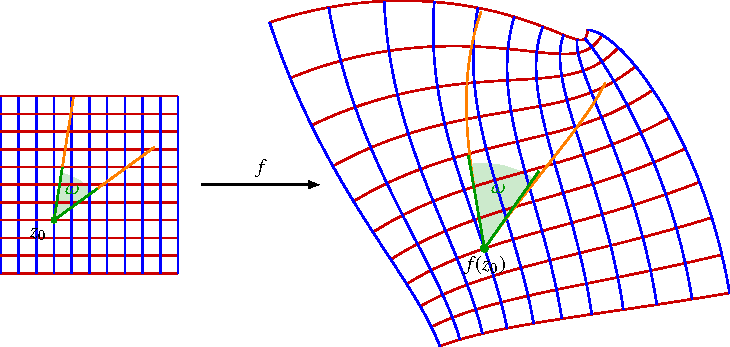
\includegraphics{chapters/020-holomorph/images/konform.pdf}
\caption{Eine holomorph Abbildung $f\colon \mathbb{C}\to\mathbb{C}$
ist konform.
Geraden mit Richtung $w\in\mathbb{C}$, $|w|=1$, durch den Punkt $z_0$
werden auf Kurven ({\color{orange}orange}) durch den Punkt $f(z_0)$
abgebildet, deren Tangenten ({\color{darkgreen}grün}) die Richtung
von $f'(z_0)\cdot w$ haben.
Die Multiplikation mit $f'(z_0)$ ist eine Drehstreckung, die Winkel
erhält.
\label{buch:holomorph:fig:konform}}
\end{figure}
%
Wir betrachten eine holomorphe Abbildung $f\colon U\to\mathbb{C}$ einer
offenen Menge nach $\mathbb{C}$.
Ein Punkt $z_0 \in U$ wird auf $f(z_0)\in\mathbb{C}$ abgebildet.
Die Abbildung~\ref{buch:holomorph:fig:konform} zeigt eine solche Abbildung.
Eine Gerade durch den Punkt $z_0$ kann durch die Richtung $d\in\mathbb{C}$
mit $|d|=1$ geschrieben werden.
Die Gerade besteht aus den Punkten $z_0+dt$ mit $t\in\mathbb{R}$.
Die Bildkurven sind $t\mapsto f(z_0+dt)$.
Die Tangente an die Bildkurve im Punkt $f(z_0)$ hat gemäss der
Ableitung  die Richtung von
\[
f'(z_0) \cdot d.
\]
Da Multiplikation mit $f'(z_0)$ eine Drehstreckung beschreibt, werden
Geraden durch $z_0$, die einen Winkel $\omega$ einschliessen, auf zwei
Tangenten abgebildet, die ebenfalls den Winkel $\omega$ einschliessen.
Folglich bleiben Winkel bei der Abbildung $f$ erhalten, sie ist
\emph{winkeltreu}.
\index{winkeltreu}%

\begin{definition}[konforme Abbildung]
Eine Abbildung, die in jedem Punkt winkeltreue ist,
heisst \emph{konform}.
\index{konform}%
\end{definition}

\begin{satz}
Eine holomorphe Funktion $f\colon U\to\mathbb{C}$ beschreibt in jedem
Punkt $z$, in dem $f'(z)\ne 0$ ist, eine konforme Abbildung.
\end{satz}

Die Gitterlinien stehen im Definitionsgebiet senkrecht aufeinander.
Die rechten Winkel werden von $f$ auf rechte Winkel zwischen den
Bildkurven der Gitterlinien abgebildet.
Daher schneiden sich die Gitterlinien in
Abbildung~\ref{buch:holomorph:fig:konform}
orthogonal.

%
% Nullstellen der Ableitung
%
\subsubsection{Nullstellen der Ableitung}
Bei einer Nullstelle von $f'(z_0)$ sind die Tangentenrichtungen der 
Bildkurven nicht definiert.
Entsprechend ist es nicht sinnvoll davon zu sprechen, dass Winkel bei
der Abbildung erhalten bleiben.
Die Abbildung $z\mapsto f(z) = z^n$ hat in Polarkoordinaten die
Darstellung 
\[
f(re^{i\varphi})
=
r^n e^{in\varphi}
=
r^n(\cos n\varphi + i\sin n\varphi).
\]
Geraden durch den Nullpunkt mit Polarwinkel $\varphi$ werden auf
Geraden durch den Nullpunkt mit Polarwinkel $n\varphi$ abgebildet.
Winkel im Nullpunkt werden also mit $n$ multipliziert.

Wir werden später zeigen, dass eine holomorphe Funktion auch eine 
konvergente Potenzreihe hat.
Hat die Ableitung $f'(z)$ eine Nullstelle im Punkt $z_0$, dann hat
$ g(z) = f(z) - f(z_0) $
eine Potenzreihe, die mit
\[
g(z)
=
\frac{f''(z_0)}{2!}(z-z_0)^2 + o((z-z_0)^2)
\]
beginnt.
Im Punkt $z_0$ werden Winkel daher mit $2$ multipliziert.
Ist die $n$-te Ableitung von $f$ die erste, die im Punkt $z_0$
nicht verschwindet, dann hat $g(z)$ die Potenzreihe
\[
g(z)
=
\frac{f^{(n)}(z_0)}{n!}(z-z_0)^n + o((z-z_0)^n).
\]
Winkel im Punkte $z_0$ werden also mit $n$ multipliziert.

Verwendet man als Definitionsgebiet
$U = \mathbb{C}\setminus\{x\in\mathbb{R} \mid x < 0\}$,
dann kann $z\mapsto f(z)=z^\alpha$ für beliebige rationale $\alpha>0$
durch die Polarformel $f(re^{i\varphi})=r^\alpha e^{i\alpha\varphi}$
definiert werden.
Winkel im Punkt $0$ werden mit $\alpha$ multipliziert.

%
% Winkeltreue Abbildungen sind holomorph
%
\subsubsection{Winkeltreue, orientierungserhaltende Abbildungen sind holomorph}
Eine differenzierbare Abbildung von $U\subset\mathbb{R}^2$ nach $\mathbb{R}^2$
hat die jacobische Matrix $\Jf$ als Ableitung.
Der Winkel zwischen den beiden Vektoren $\vec{u}$ und $\vec{v}$ und
zwischen den Bildvektoren ist
\begin{equation}
\cos
\angle(\vec{u},\vec{v})
=
\frac{\vec{u}\cdot\vec{v}}{|\vec{u}|\cdot |\vec{v}|}
\qquad\text{bzw.}\qquad
\cos
\angle(\Jf \vec{u},\Jf \vec{v})
=
\frac{\Jf \vec{u}\cdot \Jf \vec{v}}{|\Jf\vec{u}|\cdot |\Jf\vec{v}|}.
\label{buch:holomorph:geometrie:coswinkel}
\end{equation}
Sie ist genau dann winkeltreu, wenn die Matrix $\Jf$ das Skalarprodukt
nur mit einem skalaren Faktor $s$ multipliziert, denn dann bleibt der
Kosinus in \eqref{buch:holomorph:geometrie:coswinkel} und damit auch
der Winkel gleich.
Dies ist gleichbedeutend mit der Matrixgleichung
\[
\Jf^t I \Jf
=
\Jf^t \Jf
=
sI
\qquad\Rightarrow\qquad
\biggl(\frac{1}{\!\sqrt{s}}\Jf\biggr)^t
\biggl(\frac{1}{\!\sqrt{s}}\Jf\biggr)
=
I.
\]
Die Matrix
\[
A = \frac{1}{\!\sqrt{s}}\Jf
=
\frac{1}{\!\sqrt{s}}
{\renewcommand{\arraystretch}{2.0}
\begin{pmatrix}
\displaystyle\frac{\partial u}{\partial x} &
\displaystyle\frac{\partial u}{\partial y} \\
\displaystyle\frac{\partial v}{\partial x} &
\displaystyle\frac{\partial v}{\partial y}
\end{pmatrix}}
\]
muss also orthogonal sein.
Ein orthogonale Matrix in zwei Dimensionen ist aber eine Drehtmatrix
oder eine Drehmatrix mit nachfolgender Spiegelung, die die Orientierung
umkehrt.
Falls $\frac{1}{\!\sqrt{s}}\Jf$ eine Drehmatrix ist, folgt
\begin{align}
\frac{1}{\!\sqrt{s}}
{\renewcommand{\arraystretch}{2.0}
\begin{pmatrix}
\displaystyle\frac{\partial u}{\partial x} &
\displaystyle\frac{\partial u}{\partial y} \\
\displaystyle\frac{\partial v}{\partial x} &
\displaystyle\frac{\partial v}{\partial y}
\end{pmatrix}}
&=
\begin{pmatrix}
\cos\varphi&-\sin\varphi\\
\sin\varphi&\phantom{-}\cos\varphi
\end{pmatrix}
\quad\Rightarrow\quad
\left\{
\renewcommand{\arraycolsep}{1.5pt}
\begin{array}{rcccl}
\displaystyle
\frac{\partial u}{\partial x}
&=&
\!\sqrt{s}\cos\varphi
&=&
\displaystyle
\frac{\partial v}{\partial y}
\\[8pt]
\displaystyle
\frac{\partial v}{\partial x}
&=&
\!\sqrt{s}\sin\varphi
&=&
\displaystyle
-\frac{\partial u}{\partial y}
\end{array}
\right.
\label{buch:holomorph:gemetrie:eqn:JfCR}
\end{align}
Die Gleichungen auf der rechten Seite von
\eqref{buch:holomorph:gemetrie:eqn:JfCR}
sind die Cauchy-Riemann-Differential\-glei\-chun\-gen.
\index{Cauchy-Riemann-Differentialgleichungen}%
Damit haben wir den folgenden Satz bewiesen.

\begin{satz}
Ist 
\[
F
\colon
U \to \mathbb{R}^2
:
(x,y) \mapsto \begin{pmatrix} u(x,y)\\v(x,y)\end{pmatrix}
\]
eine differenzierbare Abbildung, die orientierungserhaltend und
winkeltreu ist.
Dann ist die Funktion $f(x+iy) = u(x,y) + iv(x,y)$ eine holomorphe
Funktion.
\end{satz}


%
% 22-riemann.tex -- Der Abbildungssatz von Riemann
%
% (c) 2026 Prof Dr Andreas Müller
%
\subsection{Der Abbildungssatz von Riemann}
Isometrische Abbildungen sind konform, bilden aber ein Gebiet immer
auf ein kongruentes Gebiet ab.
Ähnlichkeitsabbildungen bilden ein Gebiet immer auf ein ähnliches
Gebiet ab.
In beiden Fällen gibt es einen sehr einfachen Zusammenhang zwischen
Urbildmenge und Bildmenge, es ist leicht zu entscheiden,
ob eine Abbildung zuwischen zwei Mengen existiert.

Die Menge der konformen Abbildung ist jedoch viel grösser,
mithilfe holomorpher Abbildungen lassen sich Abbildungen
zwischen sehr viel allgemeineren Gebieten der komplexen Ebene
konstruieren.
Wir definieren den folgenden Begriff, um die Idee der
bijektiven, winkeltreuen und orientierungserhaltenden Abbildung
für komplexe Funktionen zu kodifizieren.

\begin{definition}[biholomorph]
Sind $U$ und $V$ offene Mengen in $\mathbb{C}$, dann heisst
eine Abbildung $f\colon U\to V$ \emph{biholomorph}, wenn sie bijektiv
und holomorph ist.
\index{biholomorph}%
\end{definition}

%
% Die obere Halbebene und Polygone
%
\subsubsection{Die obere Halbebene und Polygone}
Die Abbildung $z\mapsto z^\alpha$ ist holomorph auf der oberen Halbebene
\[
H = \{z\in\mathbb{C}\mid \operatorname{Im}z> 0\}.
\]
\index{obere Halbebene}%
\index{Halebene, obere}%
Sie bildet die reelle Achse auf zwei Geraden ab, die den Winkel $\alpha \pi$
einschliessen.
Durch Zusammensetzen solcher Abbildungen lässt sich eine Abbildung
der oberen Halbebene auf ein Polygon konstruieren.

\begin{definition}[Schwarz-Christoffel-Transformation]
Für reelle Zahlen $a_k$ mit $a_1<a_2<\dots<a_n$, Winkel
$\alpha_1,\dots,\alpha_n\in\mathbb{R}$ und eine Konstante $K\in \mathbb{C}$
heisst die auf der oberen Halbebene definierte Abbildung
\[
z
\mapsto 
f(z)
=
\int^z \frac{K}{
(w-a_1)^{1-\alpha_1/\pi}
(w-a_2)^{1-\alpha_2/\pi}
\dots
(w-a_n)^{1-\alpha_n/\pi}
}\,dw
\]
die Schwarz-Christoffel-Transformation.
\index{Schwarz-Christoffel-Transformation}%
\end{definition}

Die Schwarz-Christoffel-Transformation ist nur bis auf eine
Integrationskonstante definiert.
Ebenso muss man bei der Berechnung der Potenzen $(w-a_k)^{1-\alpha k/\pi}$
im Nenner eine geeignete Fortsetzung der Potenzfunktion wählen, damit
eine holomorphe Funktion entsteht.

Man kann zeigen, dass die Schwarz-Christoffel-Transformation die reelle Achse
auf ein Polygon mit Innenwinkeln $\alpha_1$ an der Stelle $f(a_i)$ abbildet.
Die Konstante $K$ kann dazu verwendet werden, das Polygon beliebig zu drehen
und zu skalieren.
Durch Wahl einer geeigneten Integrationskonstante kann das Polygon an
jede beliebige Stelle der komplexen Ebene verschoben werden.

Ein bekannter Spezialfall der Schwarz-Christoffel-Transformation ist
das elliptische Integral
\begin{align*}
f(z)
&=
\int^z
\frac{1}{\!\sqrt{(1-w^2)(1-k^2w^2)}}\,dw
\\
&=
\int^z 
\frac{1/k^2}{\!\sqrt{(w^2-1)(k^2w^2-\frac{1}{k^2})}}\,dw
\\
&=
\int^z
\frac{1/k^2}{
(w-1)^{1-\frac12}
(w-\frac{1}{k})^{1-\frac12}
(w+\frac{1}{k})^{1-\frac12}
(w+1)^{1-\frac12}
}\,dw.
\end{align*}
mit $0<k<1$.
Die Bildmenge ist ein Polygon mit 5 Ecken und Winkeln $90^\circ$-Winkeln
in den Ecken $f(\pm 1)$ und $f(\pm\frac{1}{k})$.
Da die Winkelsumme in einem 5-Eck $540^\circ$ ist, muss der Winkel
an der Ecke $\lim_{z\to\infty}f(z)$ $180^\circ$ sein.
Mehr Information zur Theorie der elliptischen Integrale findet der
interessierte Leser in Kapitel~\ref{chapter:elliptisch}.

Das Beispiel der elliptischen Integrale zeigt, dass man nicht erwarten
kann, die Transformation in geschlossener Form auszuführen.
Für die numerische Rechnung ist die Definition durch die Differentialgleichung
\[
\frac{f''(z)}{f'(z)}
=
\sum_{k=1}^n \frac{\alpha_k-1}{z-a_k}
\]
oft zugänglicher.
In Matlab steht ein Paket zur Verfügung, welches die
Schwarz-Christoffel-Transformation durch interaktive Wahl der Eckpunkte
des Polygons zu konstruieren gestattet.
\index{Matlab}%
Sie wird in Kapitel~\ref{chapter:elektro} verwendet.

%
% Der riemannsche Abbildungssatz
%
\subsubsection{Der riemannsche Abbildungssatz}
Die Schwarz-Christoffel-Transformation ist eine diskrete Approxomation
des folgenden allgemeine Satzes, der zum ersten Mal von
Bernhard Riemann
\index{Riemann, Bernhard}%
in seiner Dissertation formuliert wurde.

\begin{definition}[Einheitskreisscheibe]
Die \emph{Einheitskreisscheibe} in der komplexen Ebene ist die offene Menge
\[
D
=
\{
z\in\mathbb{C}
\mid
|z|<1
\}.
\]
\end{definition}

\begin{satz}[Riemann]
\label{buch:holomorph:riemann:satz:riemann}
Ist $U$ ein einfach zusammenhängendes Gebiet in $\mathbb{C}$, welches nicht
ganz $\mathbb{C}$ ist, dann gibt es eine biholomorphe Abbildung
$f\colon U\to D$ von $U$ auf die Einheitskreisscheibe.
Die Abbildung ist eindeutig bestimmt, wenn zusätzlich von einem Punkt
$z_0\in H$ gefordert wird, dass $f(z_0)=0$ und $f'(z_0)>0$ verlangt wird.
\end{satz}

Der von Riemann in seiner Dissertation im Jahr 1851 gegeben Beweis
wurde später von Weierstrass als unvollständig erkannt.
\index{Weierstrass, Karl}%
Den ersten vollständigen Beweis gab William Fogg Osgood erst 1900.
\index{Osgood, William Fogg}%
Ein Beweis würde den Rahmen dieses Seminars sprengen, viele Standardwerke
über komplexe Analysis wie \cite{buch:alfohrs,buch:lang} enthalten
Beweise des Satzes.

Auch die Einheitskreisscheibe erfüllt die Voraussetzungen des Satzes.
Drehungen $z \mapsto f(z)=e^{i\varphi} z$ bilden $D$ biholomorph auf $D$ ab.
Die Forderung $f'(z)=e^{i\varphi}>0$ in der Formulierung des
Satzes~\ref{buch:holomorph:riemann:satz:riemann}
bedeutet, dass $\varphi=0$ sein muss,
sie schliesst also Drehungen aus.

Für $z_0\in D$ ist die Abbildung
\begin{equation}
z
\mapsto
f(z)
=
e^{i\varphi}\frac{z-z_0}{1-\bar{z}_0z}
\label{buch:holomorph:geometrie:automorphD}
\end{equation}
als rationale Funktion holomorph.
Sie bildet $z_0$ auf den Nullpunkt ab.
Für einen Punkt $z$ auf dem Rand von $D$ ist $|z|=1$ und daher.
\[
1-\bar{z}_0z
=
|z|^2-\bar{z}_0z
=
\bar{z}z-\bar{z}_0z
=
(\bar{z}-\bar{z}_0)z.
\]
Dies bedeutet, dass $f(z)$ den Betrag
\[
|f(z)|^2
=
\frac{|z-z_0|^2}{|1-\bar{z}_0z|^2}
=
\frac{|z-z_0|^2}{|(\bar{z}-\bar{z}_0)z|^2}
=
\frac{|z-z_0|^2}{|\bar{z}-\bar{z}_0|^2\,|z|^2}
=
\frac{|z-z_0|^2}{ |z-z_0|^2}
=
1
\]
hat.
Der Rand von $D$ wird also wieder auf den Rand von $D$ abgebildet.
Der Faktor $e^{i\varphi}$ fügt eine Drehung um den Winkel $\varphi$ hinzu.
Sie ist auch umkehrbar:
\begin{align*}
w &= e^{i\varphi}\frac{z-z_0}{1-\bar{z}_0z}
&&\Rightarrow&
we^{-i\varphi}(1-\bar{z}_0z) &= z-z_0
\\
&&&&
we^{-i\varphi} + z_0 &= z+we^{-i\varphi}\bar{z}_0z
\\
&&&&
we^{-i\varphi} + z_0 &= z(1+we^{-i\varphi}\bar{z}_0)
\\
&&&&
z&=
\frac{1+we^{-i\varphi}\bar{z}_0}{ we^{-i\varphi} + z_0}.
\end{align*}
Poincaré hat gezeigt, dass jede biholomorphe Selbstabbildung von $D$
die Form \eqref{buch:holomorph:geometrie:automorphD} hat.
Dies erklärt, warum die Zusatzbedingung des Satzes von Riemann, dass
$z_0\in U$ auf $0$ abgebildet werden muss, die Abbildung eindeutig macht.

Die obere Halbebene $H$ erfüllt die Voraussetzungen des riemannschen
Abbildungssatzes.
Er garantiert, dass es eine Abbildung $f\colon H\to D$ der oberen
Halbebene auf die Einheitskreisscheibe gibt.
Eine solche kan als Möbius-Transformation gefunden werden, wie in
Kapitel~\ref{chapter:moebius} gezeigt wird.
Auch ein Polygon $P$ in der komplexen Ebene erfüllt die Bedingungen,
somit gibt es auch ein biholomorphe Abbildung des Polygons auf die
Einheitskreisscheibe.
Die Zusammensetzung $g^{-1}\circ f$ ist dann eine biholomorphe Abbildung
der oberen Halbebene auf das Polygon.
Die Schwarz-Christoffel-Transformation ist eine explizite Formel
für diese Abbildung.

%
% 23-anwendungen.tex -- Anwendungen
%
% (c) 2026 Prof Dr Andreas Müller
%
\subsection{Anwendungen
\label{buch:holomorph:geometrie:subsection:anwendungen}}
Konforme Abbildungen ermöglichen, komplizierte Gebiete auf 
komplex differenzierbare Art auf sehr einfache Gebiete abzubilden.
Zum Beispiel kann man nach einer harmonischen Funktion mit 
gegebenen Randwerten auf dem Gebiet fragen.
Die konforme Abbildung macht daraus das Problem, eine harmonische
Funktion auf einem Kreisgebiet mit gegebenen Randwerten zu finden.
Für Lösung dieses Problem gibt es aber sogar eine Formel von Poisson.
Durch Zusammensetzen der Lösung von Poisson mit der konformen
Abbildung entsteht eine Lösung des schwierigen Problems auf dem
ursprünglichen Gebiet.

Diese Idee, durch Abbildung des Gebietes eine Aufgabenstellung
auf eine bereits gelöste Aufgabe zu transformieren, wird in
zwei weiteren Kapiteln dieses Seminars verwendet.
In Kapitel~\ref{chapter:elektro} wird die Elektrostatik in der
Ebene untersucht.
Da in der Elektrostatik alles durch das elektrostatische Potential
gegeben ist, genügt es Potentialfunktionen zu finden.
Für komplexe Geometrie der berandenden Leiter kann dies eine
sehr schwierige Aufgabe sein.
Das Potential eines unregelmässigen Körpers kann aber durch
eine Abbildung der Ebene ausserhalb des Körpers auf das
äussere der Einheitskreisscheibe gefunden werden,
da das Potential eines Kreises $\sim\frac1r$ ist.

Zweidimensionale laminare Strömungen lassen sich durch die sogenannte
Stromfunktion beschreiben, die eine harmonische Funktion ist.
Es ist jedoch im allgemeinen schwierig, diese Funktion für eine
komplexe Geometrie des umströmten Körpers, zum Beispiel eines Flügelprofils,
zu finden.
Für die Umströmung eines Kreises kann man jedoch eine Formel
angeben.
Es muss jetzt nur noch eine Abbildung des Aussenraumes des Flügelprofils
auf den Aussenraum des Kreises gefunden werden.
Diese Idee ermöglicht sogar eine Formel für den Auftrieb eines Flügels
herzuleiten, sie wird in Kapitel~\ref{chapter:joukowski} genauer
ausgeführt.




%
% 3-nichtholomorph.tex
%
% (c) 2025 Prof Dr Andreas Müller
%
\section{Nicht holomorphe Funktionen
\label{buch:holomorph:section:nichtholomorph}}
\kopfrechts{Nicht holomorphe Funktionen}
Die Cauchy-Riemann-Differentialgleichungen zeigen, dass nicht jede
Funktion, die als Funktion $\mathbb{R}^2\to\mathbb{R}^2$ betrachtet
differenzierbar ist, auch holomorph ist.
In diesem Abschnitt soll eine weitere Charakterisierung holomorpher
Funktionen gezeigt werden.

%
% 31-zbarz.tex -- Funktionen von $z$ und $\bar{z}$
%
% (c) 2026 Prof Dr Andreas Müller
%
\subsection{Funktionen von $z$ und $\bar{z}$}
Bisher haben wir zur Berechnung der Ableitung einer komplexen Funktion
$f(z)$ als Funktionen der reellen Variablen $x$ und $y$ mit $z=x+iy$
betrachtet.
Die Funktion $z\mapsto \operatorname{Re}z=x$ und
$z\mapsto \operatorname{Im}z=y$ können als reellwertige Funktionen
nicht holomorph sein.
Die gleiche Information, die in $x$ und $y$ steckt, lässt sich aber auch
aus $z$ und $\bar{z}$ herausholen.
Da $z\mapsto z$ ganz offensichtlich eine holomorphe Funktion ist, scheint
dies eine vorteilhaftere Parametrisierung zu sein.

%
% z und \bar{z} als unabhängige Variablen
%
\subsubsection{$z$ und $\bar{z}$ als unabhängige Variablen}
Die Potenzfunktionen $z\mapsto z^k$ und alle Funktionen, die sich als 
Potenzreihen in $z$ ausdrücken lassen, konnten dank der Rechenregeln für
die komplexe Ableitung sehr leicht als holomorph erkannt werden.
Für Funktionen, die nur durch Realteil $u(x,y)$ und Imaginärteil $v(x,y)$
von Real- und Imaginärteil von $z$ ausgedrückt sind, mussten die
Cauchy-Riemann-Differentialgleichungen beigezogen werden, um Holomorphie
zu entscheiden.
Wir versuchen diese Vorgehensweise dadurch zu vereinfachen, dass wir
$z$ und $\bar{z}$ als unabhängige Variablen verwenden.

Für die Umrechnung zwischen $x$-$y$-Parametern und $z$-$\bar{z}$-Parametern
verwenden wir die Beziehungen
\begin{equation}
\left.
\begin{aligned}
     z  &= x + iy \\
\bar{z} &= x - iy 
\end{aligned}
\right\}
\qquad\Leftrightarrow\qquad
\left\{
\begin{aligned}
x &= \frac12    (z + \bar{z}) \\
y &= \frac1{2i} (z - \bar{z})
\end{aligned}
\right.
\label{buch:holomorph:nichtholomorph:eqn:xyzzbar}
\end{equation}

\begin{beispiel}
Wir betrachten die Funktion $f(z) = u(x,y)+iv(x,y)$ mit
$u(x,y)=x^2-y^2$ und $v(x,y)=2xy$.
Ersetzen wir mit Hilfe der Formeln
\eqref{buch:holomorph:nichtholomorph:eqn:xyzzbar}
die Variablen $x$ und $y$ durch $z$ und $\bar{z}$, dann ist
\begin{align*}
u(x,y)
&=
\frac14(z^2 + 2z\bar{z} + \bar{z}^2)
-
\frac1{-4}(z^2 - 2z\bar{z} + \bar{z}^2)
=
\frac14(2z^2 + 2\bar{z}^2)
\\
v(x,y)
&=
2
\frac1{4i}(z + \bar{z})(z - \bar{z})
=
\frac{1}{2i}(z^2 - \bar{z}^2)
\\
f(z)
&=
\frac12(z^2+\bar{z}^2)
+
\frac12(z^2-\bar{z}^2)
=
z^2.
\end{align*}
Die Rechnung hat also gezeigt, dass $f(z)$ sich auch allein als eine
Funktion von $z$ ausdrücken lässt, die Variable $\bar{z}$ wird nicht
gebraucht, um einen algebraischen Ausdruck für $f(z)$ zu konstruieren.
\end{beispiel}

\begin{beispiel}
\label{buch:holomorph:nichtholomorph:bsp:bbetrag2}
Wenden wir
\eqref{buch:holomorph:nichtholomorph:eqn:xyzzbar}
auf die Funktion $f(z) = x^2 + y^2$ 
an, erhalten wir
\begin{align*}
f(z)
&=
\frac14(z+\bar{z})^2
+
\frac1{-4}(z-\bar{z})^2
=
\frac14\bigl(
z^2 + 2z\bar{z} + \bar{z}^2
-
(z^2 - 2z\bar{z} + \bar{z}^2)
\bigr)
=
z\bar{z}.
\end{align*}
Die Funktion $f(z)=x^2+y^2=|z|^2$ lässt sich also nicht allein mit
$z$ ausdrücken.
\end{beispiel}

Wenn der Imaginärteil der Funktion $f(z)$ verschwindet, müsste nach den
Cauchy-Riemann-Differentialgleichungen 
\[
\frac{\partial u}{\partial x} = 0
\qquad\text{und}\qquad
\frac{\partial u}{\partial y} = 0
\]
sein, somit dürfte $u$ weder von $x$ noch von $y$ abhängen, $f(z)$ müsste
eine reelle Konstante sein, wenn Sie holomorph sein sollte.
Die Funktion von Beispiel~\ref{buch:holomorph:nichtholomorph:bsp:bbetrag2}
kann also nicht holomorph sein.

%
% Ableitungen nach $z$ und $\bar{z}$
%
\subsubsection{Ableitungen nach $z$ und $\bar{z}$}
Verschwindet eine partielle Ableitung einer Funktion von mehreren
reellen Variablen, dann bedeutet dies, dass die Funktion nicht
von der betreffenden Variable abhängt.
Es muss also einen Ausdruck geben, in dem diese Variable gar nicht
vorkommt.
Die Beispiele des vorangegangenen Abschnittes haben angedeutet, dass 
eine holomorphe Funktion nicht von $\bar{z}$ sondern nur von $z$ abhängt.
Es stellt sich daher die Frage, ob man diese Eigenschaft auch durch das
Verschwinden einer Art partieller Ableitung nach $\bar{z}$ ausdrücken
kann.

In
Abschnitt~\ref{buch:holomoprh:holomorph:subsection:komplexedifferenzierbarkeit}
wurde gezeigt, dass die komplexe Ableitung sowohl durch Ableiten
nach dem Realteil wie auch nach dem Imaginärteil gefunden werden
kann.
Es wurde gefunden, dass
\[
\frac{df}{dz}
=
\frac{\partial f}{\partial x}
=
\frac{1}{i}
\frac{\partial f}{\partial y}
=
-i\frac{\partial f}{\partial y}
\]
ist.
Zwar lässt sich die komplexe Ableitung mit diesen Formeln oft sehr
leicht berechnen.
Aus mathematischer Sicht sind sie jedoch nicht sehr schön, da sie den
Real- bzw.~den Imaginärteil bevorzugen.
Dies kann durch Bildung des Mittelwertes vermieden werden, es ist nämlich
\begin{equation}
\frac{df}{dz}
=
\frac{1}{2}
\biggl(
\frac{\partial f}{\partial x}
-i
\frac{\partial f}{\partial y}
\biggr).
\label{buch:holomorph:nichtholomorph:eqn:partialddz}
\end{equation}
Setzt man die Zerlegung $f=u+iv$ in Real- und Imaginärteil ein, kann
man mit den Cauchy-Riemann-Differentialgleichungen die ursprünglichen
Formeln zurückgewinnen:
\begin{align*}
\frac12
\biggl(
\frac{\partial f}{\partial x}
-i
\frac{\partial f}{\partial y}
\biggr)
&=
\frac12
\biggl(
\frac{\partial u}{\partial x}+i\frac{\partial v}{\partial x}
-
i
\biggl(
\frac{\partial v}{\partial y} + i\frac{\partial v}{\partial y}
\biggr)
\biggr)
=
\frac12
\biggl(
\frac{\partial u}{\partial x}
+
\frac{\partial v}{\partial y}
\biggr)
+
\frac{i}2
\biggl(
\frac{\partial v}{\partial x} - \frac{\partial u}{\partial y}
\biggr)
\\
&=
\begin{cases}
\displaystyle
\frac12
\biggl(
\frac{\partial u}{\partial x}
+
{\color{darkred}\frac{\partial u}{\partial x}}
\biggr)
+
\frac{i}2
\biggl(
\frac{\partial v}{\partial x}
+
{\color{darkred}\frac{\partial v}{\partial x}}
\biggr)
=
\frac{\partial f}{\partial x}
&\quad
\text{aus
$\displaystyle
\frac{\partial v}{\partial y}
=
{\color{darkred}
\frac{\partial u}{\partial x}}$
und
$\displaystyle
\frac{\partial u}{\partial y}
=
{\color{darkred}-\frac{\partial v}{\partial x}}$,}
\\[10pt]
\displaystyle
\frac12\biggl(
{\color{darkred}\frac{\partial v}{\partial y}}
+
\frac{\partial v}{\partial y}
\biggr)
+
\frac{i}2\biggl(
{\color{darkred}-\frac{\partial u}{\partial y}}
-
\frac{\partial u}{\partial y}
\biggr)
=
\frac{1}{i}
\frac{\partial f}{\partial y}
&\quad
\text{aus
$\displaystyle
\frac{\partial u}{\partial x}
=
{\color{darkred}\frac{\partial v}{\partial y}}
$
und
$\displaystyle
\frac{\partial v}{\partial x}
=
{\color{darkred}-\frac{\partial u}{\partial y}}
$.}
\end{cases}
\end{align*}
Die Cauchy-Riemann-Differentialgleichungen zeigen also, dass der 
``partielle'' Ableitungsoperator $\partial/\partial z$ mit dem
komplexen Ableitungsoperator $d/dz$ übereinstimmt.

Die Definition
\eqref{buch:holomorph:nichtholomorph:eqn:partialddz}
suggeriert, dass man auch den ``konjugiert konplexen'' Operator
\begin{equation}
\frac{\partial}{\partial\bar{z}}
=
\frac12\biggl(
\frac{\partial}{\partial x}
+
i
\frac{\partial}{\partial y}
\biggr)
\end{equation}
definieren kann.
Angewendet auf eine komplexe Funktion $f=u+iv$ lautet er
\[
\frac{\partial f}{\partial \bar{z}}
=
\frac12
\biggl(
\frac{\partial u}{\partial x} + i\frac{\partial v}{\partial x}
+
i\frac{\partial u}{\partial y} - \frac{\partial v}{\partial y}
\biggr)
=
\frac12\biggl(
\frac{\partial u}{\partial x}
-
\frac{\partial v}{\partial y}
\biggr)
+
\frac{i}2\biggl(
\frac{\partial v}{\partial x}
+
\frac{\partial u}{\partial y}
\biggr).
\]
Die Cauchy-Riemann-Differentialgleichungen ermöglichen, dem Real-
und Imaginärteil
\begin{align*}
\frac{\partial u}{\partial x}
&=
\frac{\partial v}{\partial y}
&&\Rightarrow&
\frac{\partial u}{\partial x}-\frac{\partial v}{\partial y}
&=
\operatorname{Re}
\frac{\partial f}{\partial\bar{z}}
=
0
\\
\frac{\partial u}{\partial y}
&=
-\frac{\partial v}{\partial x}
&&\Rightarrow&
\frac{\partial v}{\partial x}
+
\frac{\partial u}{\partial y}
&=
\operatorname{Im}\frac{\partial f}{\partial\bar{z}}
=
0
\end{align*}
einen Sinn zu geben.
Wenn sowohl Realteil wie auch Imaginärteil von $\partial f/\partial\bar{z}$
verschwinden, ist die Funktion holomorph.
Die Notation als partielle Ableitung suggeriert, dass eine holomorphe
Funktion nicht von $\bar{z}$ abhängt, sondern nur von $z$.

\begin{beispiel}
Die Funktion $z\mapsto z$ hat Realteil $u(x,y)=x$ und $v(x,y)=y$
mit den partiellen Ableitungen
\[
\frac{\partial z}{\partial x} = 1 
\quad\text{und}\quad
\frac{\partial z}{\partial y} = i
\qquad\Rightarrow\qquad
\left\{
\begin{aligned}
\frac{\partial z}{\partial z}
&=
\frac12
\biggl(
\frac{\partial z}{\partial x}
-i
\frac{\partial z}{\partial y}
\biggr)
=
\frac{1}{2}
(1+1)
=
1,
\\
\frac{\partial z}{\partial\bar{z}}
&=
\frac12
\biggl(
\frac{\partial z}{\partial x}
+i
\frac{\partial z}{\partial y}
\biggr)
=
\frac12(1-1)
=
0.
\end{aligned}
\right.
\]
Wie erwartet zeigt die verschwindende partielle Ableitung nach $\bar{z}$,
dass die Funktion holomorph ist.
\end{beispiel}

\begin{beispiel}
Die Funktion $z\mapsto\bar{z}$ hat Realteil $u(x,y)=x$ und
Imaginärteil $v(x,y)=-y$ und damit die partiellen Ableitungen
\[
\frac{\partial \bar{z}}{\partial x} = 1 
\quad\text{und}\quad
\frac{\partial \bar{z}}{\partial y} = -i
\qquad\Rightarrow\qquad
\left\{
\begin{aligned}
\frac{\partial \bar{z}}{\partial z}
&=
\frac12
\biggl(
\frac{\partial z}{\partial x}
-i
\frac{\partial z}{\partial y}
\biggr)
=
\frac12 (1-1)
=
0,
\\
\frac{\partial \bar{z}}{\partial \bar{z}}
&=
\frac12
\biggl(
\frac{\partial\bar{z}}{\partial x}
+i
\frac{\partial\bar{z}}{\partial y}
\biggr)
=
\frac12(1+1)
=
1.
\end{aligned}
\right.
\]
Die partielle Ableitung nach $\bar{z}$ verschwindet nicht, also
sind die Cauchy-Riemann-Diffe\-rentialgleichung nicht erfüllt, sie
kann also nicht holomorph sein.
\end{beispiel}

Wir fassen die Erkenntnisse dieses Abschnitts wie folgt zusammen.

\begin{definition}[Wirtinger-Ableitung]
Die partiellen Ableitungen einer komplexen Funktion $f\colon U\to\mathbb{C}$
mit $U\subset\mathbb{C}$ sind definiert durch die partiellen Ableitungen
nach Realteil $x$ und Imaginärteil $y$ der komplexen Variable $z=x+iy$
durch
\begin{align*}
\frac{\partial}{\partial z}
&=
\frac12\biggl(
\frac{\partial}{\partial x}
-i
\frac{\partial}{\partial y}
\biggr)
&&\text{und}&
\frac{\partial}{\partial\bar{z}}
&=
\frac12\biggl(
\frac{\partial}{\partial x}
+i
\frac{\partial}{\partial y}
\biggr).
\end{align*}
Sie heissen auch die \emph{Wirtinger-Ableitungen}.
\index{Wirtinger-Ableitung}%
Umgekehrt ist
\[
\frac{\partial}{\partial x}
=
\frac{\partial}{\partial z}
+
\frac{\partial}{\partial\bar{z}}
\qquad\text{und}\qquad
\frac{\partial}{\partial y}
=
i
\biggl(
\frac{\partial}{\partial z}
-
\frac{\partial}{\partial\bar{z}}
\biggr)
\]
Eine Funktion heisst \emph{holomorph}, wenn sie als Funktion zweier
reeller Variablen differenzierbar ist und ausserdem die partielle
Ableitung nach $\bar{z}$
\[
\frac{\partial f}{\partial \bar{z}}
=
0
\]
verschwindet.
\end{definition}

Die konjugiert komplexe Funktion $\bar{f}$ hat die komplexen
Ableitungen
\begin{equation}
\begin{aligned}
\frac{\partial \bar{f}}{\partial z}
&=
\frac12
\biggl(
\frac{\partial u}{\partial x}
-
i
\frac{\partial v}{\partial x}
-
i
\biggl(
\frac{\partial u}{\partial y}
-i
\frac{\partial v}{\partial y}
\biggr)
\biggr)
=
\frac12\biggl(
\frac{\partial u}{\partial x}-\frac{\partial v}{\partial y}
\biggr)
-
\frac{i}2
\biggl(
\frac{\partial u}{\partial y}
+
\frac{\partial v}{\partial x}
\biggr)
=
\overline{\biggl(
\frac{\partial f}{\partial \bar{z}}
\biggr)}
\\
\frac{\partial \bar{f}}{\partial \bar{z}}
&=
\frac12
\biggl(
\frac{\partial u}{\partial x} - i \frac{\partial v}{\partial x}
+
i
\biggl(
\frac{\partial u}{\partial y} - i \frac{\partial v}{\partial y}
\biggr)
\biggr)
=
\frac12
\biggl(
\frac{\partial u}{\partial x}
+
\frac{\partial v}{\partial y}
\biggr)
+
\frac{i}{2}
\biggl(
\frac{\partial u}{\partial y}
-
\frac{\partial v}{\partial x}
\biggr)
=
\overline{\biggl(
\frac{\partial f}{\partial z}
\biggr)}.
\end{aligned}
\label{buch:holomorph:nichtholomorph:eqn:dkonj}
\end{equation}
Formal vertauscht der Konjugationsoperator also mit den Ableitungen,
wenn man die Variable, nach der abgeleitet wird, ebenfalls konjugiert.

%
% 32-komplexj.tex -- Jacobi-Matrix einer komplexen Funktion
%
% (c) 2026 Prof Dr Andreas Müller
%
\subsection{Die komplexe Jacobi-Matrix einer komplexen Funktion}
Die ursprünglichen Ableitungen nach $x$ und $y$ können durch Linearkombination
der beiden partiellen Ableitungsoperatoren $\partial/\partial z$ und
$\partial/\partial\bar{z}$ wiedergewonnen werden:
\begin{align*}
\frac{\partial f}{\partial x}
=
\frac{\partial u}{\partial x}
+
i\frac{\partial v}{\partial x}
&=
\frac{\partial f}{\partial z}
+
\frac{\partial f}{\partial \bar{z}}
&&\text{und}
&
-i
\frac{\partial f}{\partial y}
=
-i\frac{\partial u}{\partial y}
+
\frac{\partial v}{\partial y}
&=
\frac{\partial f}{\partial z}
-
\frac{\partial f}{\partial \bar{z}}
\end{align*}
Die partiellen komplexen Ableitungsoperatoren enthalten also die
gesamte Information, die die partiellen Ableitungen nach den reellen
Variablen $x$ und $y$ wiedergeben.

Auch der Real- und Imaginärteil einer komplexen Zahl
$\Delta z=\Delta x + i\Delta y$
lässt sich gemäss \eqref{buch:holomorph:nichtholomorph:eqn:xyzzbar}
aus $\Delta z$ und $\overline{\Delta z}=\Delta x -i\Delta y$
rekonstruieren lassen.
Die Jacobi-Matrix der Funktion $f$ betrachtet als reelle Funktion
$\mathbb{R}^2\to\mathbb{R}^2$ sollte sich also auch als eine Matrix
ausdrücken lassen, die auf den 2-dimensionalen komplexen
Vektor mit Komponenten $\Delta z$ und $\overline{\Delta z}$ wirkt.

Da wir nicht a priori davon ausgehen möchten, dass die Funktion $f$
holomorph ist, schreiben wir sie als $f(z,\bar{z})$ und untersuchen
später, was sich ergibt, wenn $f$ holomorph ist, also nicht von $\bar{z}$
abhängt.

Die reelle Jacobi-Matrix der Funktion $f(z) = u(x,y) + iv(x,y)$
ermöglicht die Konstruktion der linearen Ersatzfunktion von $f$
betrachtet als Funktion zweier reeller Variablen.
Wir verwenden Vektornotation, um diese wie folgt auszudrücken:
\begin{align*}
\begin{pmatrix}
u(x+\Delta x,y+\Delta y)\\
v(x+\Delta x,y+\Delta y)
\end{pmatrix}
&=
\begin{pmatrix}
u(x,y)\\
v(x,y)
\end{pmatrix}
+
\bgroup
\renewcommand{\arraystretch}{1.9}
\begin{pmatrix}
\displaystyle
\frac{\partial u}{\partial x}(x,y) &
\displaystyle
\frac{\partial u}{\partial y}(x,y) \\
\displaystyle
\frac{\partial v}{\partial x}(x,y) &
\displaystyle
\frac{\partial v}{\partial y}(x,y)
\end{pmatrix}
\egroup
\begin{pmatrix}
\Delta x \\
\Delta y
\end{pmatrix}
+
o(\Delta x,\Delta y)
\end{align*}
In diesem Ausdruck möchten wir alles durch die Funktionen $f(z,\bar{z})$
und ihre konjugiert komplexe Funktion $\bar{f}(z,\bar{z})$ sowie die Variablen
$z$ und $\bar{z}$ und die partiellen Ableitungen nach $z$ und $\bar{z}$
ausdrücken.
Für das Inkrement findet man
\[
\begin{pmatrix}
\Delta x\\
\Delta y
\end{pmatrix}
=
\begin{pmatrix}
\frac12   (\Delta z+\overline{\Delta z}) \\
\frac1{2i}(\Delta z-\overline{\Delta z})
\end{pmatrix}.
\]
Die Ableitungen werden
\begin{align*}
\frac{\partial u}{\partial x}
&=
\frac12
\biggl(
\frac{\partial f}{\partial x}
+
\frac{\partial \bar{f}}{\partial x}
\biggr)
=
\frac12
\biggl(
\frac{\partial f}{\partial z}
+
\frac{\partial f}{\partial \bar{z}}
+
\frac{\partial \bar{f}}{\partial z}
+
\frac{\partial \bar{f}}{\partial \bar{z}}
\biggr),
\\
\frac{\partial u}{\partial y}
&=
\frac12
\biggl(
\frac{\partial f}{\partial y}
+
\frac{\partial \bar{f}}{\partial y}
\biggr)
=
\frac12
\biggl(
i
\biggl(
\frac{\partial f}{\partial z}
-
\frac{\partial f}{\partial\bar{z}}
\biggr)
+
i
\biggl(
\frac{\partial\bar{f}}{\partial z}
-
\frac{\partial\bar{f}}{\partial\bar{z}}
\biggr)
\biggr),
\\
\frac{\partial v}{\partial x}
&=
\frac1{2i}
\biggl(
\frac{\partial f}{\partial x}
-
\frac{\partial\bar{f}}{\partial x}
\biggr)
=
\frac1{2i}
\biggl(
\frac{\partial f}{\partial z}
+
\frac{\partial f}{\partial \bar{z}}
-
\frac{\partial \bar{f}}{\partial z}
-
\frac{\partial \bar{f}}{\partial \bar{z}}
\biggr),
\\
\frac{\partial v}{\partial y}
&=
\frac1{2i}
\biggl(
\frac{\partial f}{\partial y}
-
\frac{\partial\bar{f}}{\partial y}
\biggr)
=
\frac1{2i}
\biggl(
i\biggl(
\frac{\partial f}{\partial z}
-
\frac{\partial f}{\partial\bar{z}}
\biggr)
-i
\biggl(
\frac{\partial\bar{f}}{\partial z}
-
\frac{\partial\bar{f}}{\partial\bar{z}}
\biggr)
\biggr).
\end{align*}
Im Interesse etwas kompakterer Formeln schreiben wir die partiellen
Ableitungen nach $z$ und $\bar{z}$ in der in der Theorie der partiellen
Differentialgleichungen üblichen Form durch einen Index in der Form
\begin{align*}
\frac{\partial f}{\partial z}
&=
f_z
&\text{und}&
&
\frac{\partial f}{\partial \bar{z}}
&=
f_{\bar{z}}.
\end{align*}
Damit können wir jetzt die lineare Ersatzfunktion als
\begin{align*}
u(x+\Delta x,y+\Delta y)
&\approx
\frac{\partial u}{\partial x}\Delta x
+
\frac{\partial u}{\partial y}\Delta y
\\
&=
\frac12
(
f_z
+
f_{\bar{z}}
+
\bar{f}_z
+
\bar{f}_{\bar{z}}
)
\frac12
(\Delta z + \overline{\Delta z})
+
\frac{i}2
(
f_z
-
f_{\bar{z}}
+
\bar{f}_z
-
\bar{f}_{\bar{z}}
)
\frac1{2i}
(\Delta z - \overline{\Delta z}),
\\
&=
\frac12
(
f_z + \bar{f}_z
)
\Delta z
+
\frac12
(
f_{\bar{z}} + \bar{f}_{\bar{z}}
)
\overline{\Delta z}
\\
v(x+\Delta x,y+\Delta y)
&\approx
\frac{\partial v}{\partial x}\Delta x
+
\frac{\partial v}{\partial y}\Delta y
\\
&=
\frac1{2i}
(
f_z + f_{\bar{z}} - \bar{f}_z - \bar{f}_{\bar{z}}
)
\frac12
(\Delta z + \overline{\Delta z})
+
\frac12
(
f_z - f_{\bar{z}} - \bar{f}_z + \bar{f}_{\bar{z}}
)
\frac1{2i}
(\Delta z - \overline{\Delta z})
\\
&=
\frac1{2i}
(
f_z - \bar{f}_z
)
\Delta z
+
\frac1{2i}
(
f_{\bar{z}}
-
\bar{f}_{\bar{z}}
)
\overline{\Delta z}
\intertext{schreiben, wobei dass Approximationszeichen $\approx$
immer eine Approximation bis auf einen $o$-Term bedeutet.
Die Funktionen $u$ und $v$ sind Real- und Imaginärteil der
Funktion $f$, daher kann man auch}
f(z+\Delta z, \bar{z}+\bar{\Delta z})
&=
u(x+\Delta x, y + \Delta y)
+
iv(x+\Delta x, y + \Delta y)
\\
&=
f_z\Delta z + f_{\bar{z}}\overline{\Delta z}
+
o(\Delta z, \overline{\Delta z})
\\
\bar{f}(z+\Delta z, \bar{z}+\overline{\Delta z})
&=
u(x+\Delta x, y + \Delta y)
-
iv(x+\Delta x, y + \Delta y)
\\
&=
\bar{f}_z \Delta z
+
\bar{f}_{\bar{z}}\Delta z
+
o(\Delta z, \overline{\Delta z})
\end{align*}
schreiben.
In Matrixform ist dies
\begin{align*}
\begin{pmatrix}
     f (z + \Delta z, \bar{z}+\overline{\Delta z})\\
\bar{f}(z + \Delta z, \bar{z}+\overline{\Delta z})
\end{pmatrix}
&=
\bgroup
\renewcommand{\arraystretch}{2.2}
\begin{pmatrix}
\displaystyle\frac{\partial f}{\partial z}(z,\bar{z}) &
\displaystyle\frac{\partial f}{\partial \bar{z}}(z,\bar{z}) \\
\displaystyle\frac{\partial \bar{f}}{\partial z}(z,\bar{z}) &
\displaystyle\frac{\partial \bar{f}}{\partial \bar{z}}(z,\bar{z})
\end{pmatrix}
\begin{pmatrix}
\Delta z\\
\overline{\Delta z}
\end{pmatrix}.
\egroup
\intertext{Die Matrix auf der rechten Seite kann man als eine
komplexe Form der Jacobimatrix sehen.
Wir können die rechte Seite auch als}
\frac{\partial(f,\bar{f})}{\partial(z,\bar{z})}
\begin{pmatrix}
\Delta z \\
\overline{\Delta z}
\end{pmatrix}
\end{align*}
schreiben.

Für eine holomorphe Funktion wird die komplexe Jacobi-Matrix zu
einer Diagonalmatrix.
Man beachte auch, dass
wegen \eqref{buch:holomorph:nichtholomorph:eqn:dkonj}
die Elemente der unteren Zeile der komplexen Jacobi-Matrix
durch Konjugation und Vertauschen aus den Elementen der oberen
Zeile hervorgehen.






\pagebreak
\uebungsabschnitt

\aufgabetoplevel{chapters/020-holomorph/uebungsaufgaben}
\begin{uebungsaufgaben}
\uebungsaufgabe{204}
\uebungsaufgabe{205}
\uebungsaufgabe{201}
\uebungsaufgabe{202}
\uebungsaufgabe{203}
\end{uebungsaufgaben}
\enduebungsabschnitt

